\documentclass[a4paper]{report}
\usepackage[backend=bibtex]{biblatex}
\addbibresource{refs.bib}
\usepackage[utf8]{inputenc}
\usepackage[T1]{fontenc}
\usepackage{textcomp}

\usepackage{url}

\usepackage{hyperref}
\hypersetup{
    colorlinks,
    linkcolor={black},
    citecolor={black},
    urlcolor={blue!80!black}
}

\usepackage{graphicx}
\usepackage{wrapfig}
\usepackage{adjustbox}
\usepackage{float}
\usepackage[usenames,dvipsnames]{xcolor}

\usepackage{listings}

\lstset{
    language=Python,
    basicstyle=\ttfamily\footnotesize,
    keywordstyle=\color{blue},
    stringstyle=\color{red},
    commentstyle=\color{gray},
    showstringspaces=false,
    frame=single,
    numbers=left,
    numberstyle=\tiny,
    breaklines=true,
    tabsize=4
}

% \usepackage{cmbright}

\usepackage{amsmath, amsfonts, mathtools, amsthm, amssymb}
\usepackage{mathrsfs}
\usepackage{cancel}

\newcommand\N{\ensuremath{\mathbb{N}}}
\newcommand\R{\ensuremath{\mathbb{R}}}
\newcommand\Z{\ensuremath{\mathbb{Z}}}
\renewcommand\O{\ensuremath{\emptyset}}
\newcommand\Q{\ensuremath{\mathbb{Q}}}
\newcommand\C{\ensuremath{\mathbb{C}}}
\let\implies\Rightarrow
\let\impliedby\Leftarrow
\let\iff\Leftrightarrow
\let\epsilon\varepsilon

% horizontal rule
\newcommand\hr{
    \noindent\rule[0.5ex]{\linewidth}{0.5pt}
}

\usepackage{tikz}
% \usepackage{tikzmark}
\usepackage{pgfplots}
\usepackage{tikz-cd}

\usetikzlibrary{calc, arrows.meta, positioning, angles, quotes, patterns}

% theorems
\usepackage{thmtools}
\usepackage{thm-restate}
\usepackage[framemethod=TikZ]{mdframed}
\mdfsetup{skipabove=1em,skipbelow=0em, innertopmargin=12pt, innerbottommargin=8pt}

\theoremstyle{definition}

\makeatletter

\declaretheoremstyle[
    headfont=\bfseries\sffamily\color{ForestGreen!70!black}, bodyfont=\normalfont,
    mdframed={
        linewidth=2pt,
        rightline=false, topline=false, bottomline=false,
        linecolor=ForestGreen, backgroundcolor=ForestGreen!5,
    }
]{thmgreenbox}

\declaretheoremstyle[
    headfont=\bfseries\sffamily\color{NavyBlue!70!black}, bodyfont=\normalfont,
    mdframed={
        linewidth=2pt,
        rightline=false, topline=false, bottomline=false,
        linecolor=NavyBlue, backgroundcolor=NavyBlue!5,
    }
]{thmbluebox}

\declaretheoremstyle[
    headfont=\bfseries\sffamily\color{NavyBlue!70!black}, bodyfont=\normalfont,
    mdframed={
        linewidth=2pt,
        rightline=false, topline=false, bottomline=false,
        linecolor=NavyBlue
    }
]{thmblueline}

\declaretheoremstyle[
    headfont=\bfseries\sffamily\color{RawSienna!70!black}, bodyfont=\normalfont,
    mdframed={
        linewidth=2pt,
        rightline=false, topline=false, bottomline=false,
        linecolor=RawSienna, backgroundcolor=RawSienna!5,
    }
]{thmredbox}

\declaretheoremstyle[
    headfont=\bfseries\sffamily\color{RawSienna!70!black}, bodyfont=\normalfont,
    numbered=no,
    mdframed={
        linewidth=2pt,
        rightline=false, topline=false, bottomline=false,
        linecolor=RawSienna, backgroundcolor=RawSienna!1,
    },
    qed=\qedsymbol
]{thmproofbox}

\declaretheoremstyle[
    headfont=\bfseries\sffamily\color{NavyBlue!70!black}, bodyfont=\normalfont,
    numbered=no,
    mdframed={
        linewidth=2pt,
        rightline=false, topline=false, bottomline=false,
        linecolor=NavyBlue, backgroundcolor=NavyBlue!1,
    },
]{thmexplanationbox}

\declaretheorem[numberwithin=chapter, style=thmgreenbox, name=Definition]{definition}
\declaretheorem[sibling=definition, style=thmredbox, name=Corollary]{corollary}
\declaretheorem[sibling=definition, style=thmredbox, name=Proposition]{prop}
\declaretheorem[sibling=definition, style=thmredbox, name=Theorem]{theorem}
\declaretheorem[sibling=definition, style=thmredbox, name=Lemma]{lemma}
\declaretheorem[sibling=definition, style=thmbluebox,  name=Example]{eg}
\declaretheorem[sibling=definition, style=thmbluebox,  name=Nonexample]{noneg}
\declaretheorem[sibling=definition, style=thmblueline, name=Remark]{remark}




\declaretheorem[numbered=no, style=thmexplanationbox, name=Proof]{explanation}
\declaretheorem[numbered=no, style=thmproofbox, name=Proof]{preuve}
\declaretheorem[style=thmbluebox,  numbered=no, name=Exercise]{ex}
\declaretheorem[style=thmblueline, numbered=no, name=Note]{note}

% \renewenvironment{proof}[1][\proofname]{\begin{replacementproof}}{\end{replacementproof}}

% \AtEndEnvironment{eg}{\null\hfill$\diamond$}%

\newtheorem*{uovt}{UOVT}
\newtheorem*{notation}{Notation}
\newtheorem*{previouslyseen}{As previously seen}
\newtheorem*{problem}{Problem}
\newtheorem*{observe}{Observe}
\newtheorem*{property}{Property}
\newtheorem*{intuition}{Intuition}


\declaretheoremstyle[
    headfont=\bfseries\sffamily\color{RawSienna!70!black}, bodyfont=\normalfont,
    mdframed={
        linewidth=2pt,
        rightline=false, topline=false, bottomline=false,
        linecolor=RawSienna, backgroundcolor=RawSienna!5,
    }
]{todo}
\declaretheorem[numbered=no, style=todo, name=TODO]{TODO}


\usepackage{etoolbox}

\AtEndEnvironment{vb}{\null\hfill$\diamond$}%
\AtEndEnvironment{intermezzo}{\null\hfill$\diamond$}%




% http://tex.stackexchange.com/questions/22119/how-can-i-change-the-spacing-before-theorems-with-amsthm
% \def\thm@space@setup{%
%   \thm@preskip=\parskip \thm@postskip=0pt
% }

\usepackage{xifthen}

\def\testdateparts#1{\dateparts#1\relax}
\def\dateparts#1 #2 #3 #4 #5\relax{
    \marginpar{\small\textsf{\mbox{#1 #2 #3 #5}}}
}

\def\@lesson{}%
\newcommand{\lesson}[3]{
    \ifthenelse{\isempty{#3}}{%
        \def\@lesson{Lecture #1}%
    }{%
        \def\@lesson{Lecture #1: #3}%
    }%
    \subsection*{\@lesson}
    \testdateparts{#2}
}

% fancy headers
\usepackage{fancyhdr}
\pagestyle{fancy}

% \fancyhead[LE,RO]{Gilles Castel}
\fancyhead[RO,LE]{\@lesson}
\fancyhead[RE,LO]{}
\fancyfoot[LE,RO]{\thepage}
\fancyfoot[C]{\leftmark}
\renewcommand{\headrulewidth}{0pt}

\makeatother

% figure support (https://castel.dev/post/lecture-notes-2)
\usepackage{import}
\usepackage{xifthen}
\pdfminorversion=7
\usepackage{pdfpages}
\usepackage{transparent}
\usepackage[margin=0.8in]{geometry}
\newcommand{\incfig}[1]{%
    \def\svgwidth{\columnwidth}
    \import{./figures/}{#1.pdf_tex}
}

% %http://tex.stackexchange.com/questions/76273/multiple-pdfs-with-page-group-included-in-a-single-page-warning
\pdfsuppresswarningpagegroup=1
\pgfplotsset{compat=1.11}
\usepackage{subcaption}

\author{Yehor Korotenko}

\newcommand{\scalar}[2]{\langle #1, #2 \rangle}
\newcommand{\scalair}[1]{\left\langle #1 \right\rangle}

% fancy chapters
\usepackage{lipsum}
\usepackage[Lenny]{fncychap}
\ChNameUpperCase
\ChNumVar{\fontsize{40}{42}\usefont{OT1}{ptm}{m}{n}\selectfont}
\ChTitleVar{\Large\sc}


\title{Notes du cours d'Analyse et Géometrie\\\vspace{1cm}
\Large Professeur: Christian Gérard \normalsize}
\begin{document}
\maketitle

\begin{abstract}
    Ce sont les notes prises en cours OLMA251 - Analyse et Géometrie fait par le professeur Christian Gérard. Ces notes contient l'information prises pendant les CMs, mais aussi mon opinion, comprehension et les choses apprises apart ce cours.
\end{abstract}


\tableofcontents


\chapter{Introduction}
\section{Éspaces $\R^d$  $\C^d$}
\begin{definition}
    \[
        \R^d = \{ X = (x_1, \ldots, x_d), x_i \in \R\}
    \] 
    $x_1, \ldots, x_d$ coordonnées cartésiennes de X
\end{definition}
\begin{eg}
   $d = 2$ coordonnées polaires:  
   \begin{align*}
      &x = r \cos \theta \\
        & y = r \sin \theta\\
        &0 \le r \le  \infty \quad \theta \in [0, 2\pi[
   \end{align*}
   \begin{center}
       
\begin{tikzpicture}
    % Create the axis
    \begin{axis}[
        axis lines=middle,
        xmin=-1, xmax=3,
        ymin=-1, ymax=3,
        xlabel={$x$},
        ylabel={$y$},
        axis equal,
        height=6cm
    ]
        % Draw the vector
        \addplot[->, thick, blue] coordinates {(0,0) (3,2)} node[right] {$\vec{v}$};

        % Draw x-axis projection manually
        \draw[thick] (axis cs: 0,0) -- (axis cs: 3,0);

        % Use TikZ outside \addplot for \pic
        \node (A) at (2, 0) {};
        \node (C) at ($(0,0)!0.5!(3,2)$) {};
        \node (B) at (0, 0) {};
        \node[above] (_) at ($(0,0)!0.5!(3,2)$) {$r$};
        
        \pic [draw,-, black, angle eccentricity=1.2, angle radius=1cm,"$\theta$"] {angle = A--B--C};
    \end{axis}
\end{tikzpicture}
\end{center}
\end{eg}

\begin{definition}
    $\R^d$ est un espace vectoriel sur  $\R$ 
    \begin{align*}
        &\vec{X} + \vec{Y} = (x_1 + y_1, \ldots, x_d + y_d)\\
        &\lambda X = (\lambda x_1, \ldots, \lambda x_d) \quad \lambda \in \R\\
        &\vec{0}_d = \vec{0} = (0, \ldots, 0)
    \end{align*}
\end{definition}
\begin{definition}\label{def:prod_scalaire}
    Un \textbf{produit scalaire}:
    \[
    X \cdot Y = x_1y_1 + x_2y_2 + \ldots x_dy_d = \|X\|\|Y\|\cos(\theta) \text{ (où } \theta \text{ est une angle entre } X \text{ et } Y \text{)}
    \] 
\end{definition}
\begin{intuition}
    Ce produit nous dit \textit{how closely the vectors point in the same direction} (cosinus tend vers 1 quand $\theta$ tend vers 0º, et cosinus tend vers 0 quand  $\theta$ tend vers 90º). Et ce produit nous permet d'avoir une projection de $X$ sur $Y$ par la formule:
    \[
    Proj(X) = \frac{X \cdot Y}{\|Y\|} \cdot \frac{Y}{\|Y\|}
    \] 
    $X \cdot Y$ donne la longeur de  $X$ et  $Y$ ensemble, en divisant cette longeur par  $\|Y\|$ (la longeur de $Y$) on obtient la longeur de $X$ sur Y, il nous reste de multiplier cette longeur par un vecteur unitaire(de longeur 1) qui pointe dans la même direction que  $Y$, (on l'obtient par $\frac{Y}{\|Y\|}$)
   \begin{center}
      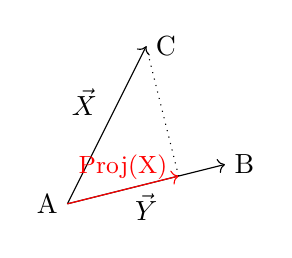
\begin{tikzpicture}
         \coordinate (A) at (0, 0); 
         \coordinate (B) at (2, 0.5);
         \coordinate (C) at (1, 2);
         \coordinate (newB) at (1.4117647059, 0.3529411765);
         \coordinate (dotBC) at (2, 1);
         \node[left] (_) at (A){A};
         \node[right] (_) at (B){B};
         \node[right] (_) at (C){C};
         \draw[->] (A) -- (B);
         \node[above left] (...) at ($(A)!0.5!(C)$) {$\vec{X}$};
         \node[below] (...) at ($(A)!0.5!(B)$) {$\vec{Y}$};
         \draw[->] (A) -- (C);
         \draw[->, red, thin] (A) -- (newB);
         \draw[dotted] (C) -- (newB);
         \node[above, red] (_) at ($(A)!0.5!(newB)$){\small Proj(X)};
      \end{tikzpicture} 
   \end{center}
\end{intuition}
\begin{prop}
    Produit scalaire respecte ces propriétés:
    \begin{enumerate}
        \item bilinaiarité $\quad \lambda \in \R$
            \begin{enumerate}
                \item $(X + Y) \cdot Z = X \cdot Z + Y \cdot Z$
                \item $(\lambda X) \cdot Z = \lambda (X \cdot Z)$
                \item $Z \cdot (X + Y) = Z \cdot X + Z \cdot Y$ 
                \item $Z \cdot (\lambda X) = \lambda (Z \cdot X)$
            \end{enumerate}
        \item symétrie $X \cdot Y = Y \cdot X$
        \item défini positif:  $X \cdot X \ge 0$ et $X \cdot X = 0 \iff X = 0_d$
    \end{enumerate}
\end{prop}
\begin{prop}
    \underline{Cauchy-Schwarz}:\\ 
    \[
        |X \cdot Y| \le (X \cdot X)^{\frac{1}{2}}(Y \cdot Y)^{\frac{1}{2}}
    \] 
\end{prop}
\begin{definition}\label{def:norm_eucl}
    La \textbf{norme euclidienne} d'un vecteur $X$ est noté:
   \[
       \|X\| = \left(\sum_{n=1}^{d} x_i^2\right)^{\frac{1}{2}} = \sqrt{x_1^2 + \ldots + x_d^2} = (X \cdot X)^{\frac{1}{2}}
   \] 
   souvent noté $\|X\|_2$
\end{definition}
\begin{intuition}
   Par le théorème de Pythogore, c'est une longeur de ce vecteur. 
\end{intuition}
\begin{prop}
    La norme suit ces propriétés:
   \begin{enumerate}
       \item $\|\lambda X\| = |\lambda|\|X\| \, X \in \R^d, \, \lambda \in \R$
       \item $\|X + Y\| \le \|X\| + \|Y\| \text{ (inégalité triangulaire)}$
       \item $\|X\| \ge 0$ et $\|X\| = 0 \iff X = 0_d$
   \end{enumerate}
\end{prop}
\begin{explanation}
    de (2)
    \begin{align*}
        \|X + Y\|^2 &= (X + Y)\cdot(X + Y) = X \cdot (X + Y) + Y \cdot (X + Y) = X \cdot X + X \cdot Y + Y \cdot X + Y \cdot Y\\
                    &= \|X\|^2 + 2X \cdot Y + \|Y\|^2 \le \|X\|^2 + 2\|X\| \|Y\| + \|Y\|^2 = (\|X\| + \|Y\|)^2
    \end{align*}
\end{explanation}
\begin{definition}
    Une \underline{norme} sur $\R^d$ est une application  $N: \: \R^d \to \R$ tell que:
    \begin{enumerate}
        \item $N(\lambda X) = |\lambda|N(X)$
        \item  $N(X + Y) \le N(X) + N(Y)$
        \item $N(X) \ge 0$ et $N(X) = 0 \iff X = 0_d$
    \end{enumerate}
\end{definition}
\begin{eg}
   \begin{align*}
       &\|X\|_1 = \sum_{n=1}^{d} |x_i|\\
       &\|X\|_{\infty} = \underset{1\le i \le n}{max} |x_i|
   \end{align*} 
\end{eg}
\section{Éspace $\C^d$}
\begin{definition}
    \[
        \C^d = \{ X = (x_1, \ldots, x_d): \: x_i \in \C\}
    \] 
    \begin{align*}
    &z \in \C \quad \overline{z} = a - ib \quad \overline{z}z = a^2 + b^2 \quad |z| = \sqrt{\overline{z}z} = \sqrt{a^2 + b^2}  \\
    &z = a + ib \qquad a = Re\,z,\,b = Im\,z\\
    &Re\,X = (Re\,x_1, \ldots, Re\,x_d) \in \R^d\\
    &Im\,X = (Im\,x_1, \ldots, Im\,x_d) \in \R^d\\
    &\underset{\in \C^d}{X} = \underset{\in \R^d}{Re\,X} + i\underset{\in \R^d}{\:Im\,X}\\
    \end{align*}
    $\C^d$ est un espace vécrotiel sur  $\C$ (même formules avec $\lambda \in \C$ corps des scalaires)
\end{definition}
\begin{definition}
    \underline{Produit scalaire:}
    \[
        (X|Y) = \sum_{n=1}^{d} \overline{x_i}y_i \in \C
    \] 
\end{definition}
\begin{prop}
   . 
   \begin{enumerate}
       \item $(X|Y)$ est "linéaire par rapport à Y"
           \begin{itemize}
               \item $(Z|X + Y) = (Z|X) + (Z|Y)$
               \item $(Z|\lambda X) = \lambda(Z|X) \quad \lambda \in \C$
               \item  $(Z|\lambda X + \mu Y) = \lambda(Z|X) + \mu(Z|Y)$
               \item  $(X + Y|Z) = (X|Z) + (Y|Z)$
               \item $(\lambda X|Z) = \overline{\lambda}(X|Z) \quad \lambda \in \C$
               \item $(\lambda X + \mu Y|Z) = \overline{\lambda}(X|Z) + \mu(Y|Z)$
           \end{itemize}
       \item $(Y|X) = \overline{(X|Y)}$
       \item $(X|X) = \sum_{n=1}^{d} \overline{x_i}x_i = \sum_{n=1}^{d} |x_i|^2$\\
           $(X|X) \ge 0$ et $(X|X) = 0 \iff X = 0_d$
   \end{enumerate}
\end{prop}
\begin{explanation}
    On a Cauchy-Schwarz:
    \begin{align*}
        (X|Y) \le (X|X)^{\frac{1}{2}}(Y|Y)^{\frac{1}{2}}
    \end{align*}
    même preuve qu'avant
\end{explanation}
On pose:
\begin{align*}
    \|X\| & \text{(ou }\|X\|_2\text{)}\\
          &= (X|X)^{\frac{1}{2}} = \left( \sum_{n=1}^{d} |x_i|^2 \right)^{\frac{1}{2}}
\end{align*}
norme hilbertienne
\[
    \underset{\in \C^d}{\|X\|^2} = \underset{\in \R^d}{\|Re\,X\|^2} + i\underset{\in \R^d}{\:\|Im\,X\|^2}\\
\] 
\begin{lemma}
   \begin{align*}
       \|X\| = \underset{\|Y\|\le 1}{sup|(X|Y)|}
   \end{align*} 
\end{lemma}
\begin{explanation}
    $|(X|Y)| \le \|X\|\|Y\| \le \|X\|$ si $\|Y\| \le 1$
    \[
    \underset{\|Y\|\le 1}{sup|(X|Y)|}
    \] 
    \underline{Autre sens:} 
    \begin{align*}
        &X \neq 0 \quad Y =  \frac{X}{\|X\|} = \lambda X \quad \lambda = \frac{1}{\|X\|}\\
        &\|Y\| = |\lambda|\|X\| = \frac{1}{\|X\|}\|X\| = 1\\
        &(X|Y) = (X|\frac{X}{\|X\|}) = \frac{1}{\|X\|}(X|X) = \|X\|\\
        &sup \{|(X|Y)|: \, \|Y\| \le  1\}\\
        &\|X\| \le sup \{|(X|Y)|: \, \|Y\|\le 1\} \quad \text{(prendre }Y = \frac{X}{\|X\|}\text{)}
    \end{align*}

\end{explanation}
\underline{Autres normes sur $\C^d$}
\begin{itemize}
    \item $\|X\|_1 = \sum_{n=1}^{d} |x_i| \quad X \in \C^d$
    \item $\|X\|_{\infty} = \underset{1\le i \le d}{sup} |x_i|$
\end{itemize}
\section{Distance sur $\R^d$}
On oublie norme et produit scalaire. On introduit la distance
\begin{definition}\label{def:distance} Une distance est une application:
    \begin{align*}
        d: \R^d &\longrightarrow \R \\
        (X, Y) &\longmapsto d((X, Y)) 
    \end{align*}
    qui suit ces propriétés:
    \begin{enumerate}
        \item $d(X, Y) = d(Y, X)$ (symétrie)
        \item $d(X, Y) \le d(X, Z) + d(Z, Y)$ (inég. triangulaire) $\forall X, Y, Z$ 
        \item $d(X, Y) \ge 0 \quad \forall X, Y$ et $d(X, Y) = 0 \iff X = Y$ 
    \end{enumerate}
\end{definition}
\begin{definition} La distance euclidienne
    \[
        d(X, Y) = \|X - Y\| = \sqrt{\sum_{n=1}^{d} (x_i - y_i)^2} 
    \] 
\end{definition}
\begin{eg} Distances
   \begin{enumerate}
       \item $d_2(X, Y) = \|X - Y\|_2$ (distance euclidienne sur $\R^d$)
       \item $d_1(X, Y) = \|X - Y\|_1$\\
           $d_{\infty}(X, Y) = \|X - Y\|_{\infty}$
       \item distance logarithmique sur $\R_+$:  $d(a, b) = |b - a|$
           \[
               \log_{10}(a) = \frac{\log(a)}{\log(10)}
           \] 
           $x, y \in ]0, +\infty[$\\ 
           $d_{\log}(x, y) = |\log_{10}(\frac{y}{x})|$ \\
           $i$ est une distance sur  $]0, +\infty[$\\
           $d_{\log}(100, 110) = \log_{10}(1,1)$
       \item distance SNCF
           \begin{center}
               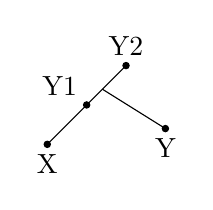
\begin{tikzpicture}
                  \coordinate (X) at (0, 0); 
                  \coordinate (Y) at (1.5, 0.2);
                  \coordinate (Y2) at (1, 1);
                  \coordinate (Y1) at ($(X)!0.5!(Y2)$);
                  \draw (X)--(Y2);
                  \draw (Y)--($(X)!0.7!(Y2)$);
                  \draw[fill=black] (X) circle (0.4mm);
                  \draw[fill=black] (Y) circle (0.4mm);
                  \draw[fill=black] (Y2) circle (0.4mm);
                  \draw[fill=black] (Y1) circle (0.4mm);
                  \node[below] (_) at (X){X};
                  \node[below] (_) at (Y){Y};
                  \node[above left] (_) at (Y1){Y1};
                  \node[above] (_) at (Y2){Y2};
               \end{tikzpicture}
               
           \end{center}
           $d(X, Y)$ distance usuelle dans  $\R^2$
           on pose:
            \begin{align*}
               \delta(X, Y) = \begin{cases}
                   d(X, Y) \text{ si } X, 0, Y \text{ alignés}\\
                   d(X, 0) + d(0, Y) \text{ sinon }
               \end{cases}
           \end{align*}
   \end{enumerate}
\end{eg}
\begin{prop}
    Soit $E$ espace métrique et deux distances $d_1$ et $d_2$. Les distances sont dites \textbf{équivalentes} si $\exists a, b \in \R$ tel que:
    \[
    \forall x, y \in E, \quad a\cdot d_1(x, y) \le d_2(x, y) \le b\cdot  d_1(x, y)
    \] 
\end{prop}

\chapter{Éspaces métriques}
\begin{definition}
    $E$ muni d'une application de distance $d$ (voir Definition \ref{def:distance}) se note  $(E, d)$: \underline{espace métrique}
\end{definition}
\begin{remark}
   si $d_1 \neq d_2$ $(E, d_1)$ n'a rien à faire avec  $(E, d_2)$ 
\end{remark}
\begin{remark}
    Retenir la version suivante de l'inégalité triangulaire:
    \[
        |d(x, z) - d(y, z)| \le d(x, y)
    \] 
\end{remark}
\begin{remark}
    \underline{Distance induite:}\\
    Si $(E, d)$ espace métrique et  $U \subset E$. Je peux restreidnre $d$ à  $U \times U$:  $(U, d)$ est aussi un éspace metrique.
\end{remark}
\section{Boules dans un espace métrique}
\begin{definition}
    $(E, d)$ espace métrique. Soit  $x_0 \in E$ et $r \ge  0$
    \begin{enumerate}
        \item $B(x_0, r) = \{ x \in E: d(x_0, x) < r$ \} boule ouverte de centre $x_0$, de rayon $r$
        \item $B_f(x_0, r) = \{ x \in E: d(x_0, x) \le  r$\} boule fermée de centre $x_0$, de rayon $r$
    \end{enumerate}
\end{definition}
\begin{figure}
    \centering
    \begin{subfigure}{0.45\textwidth}
        \centering
        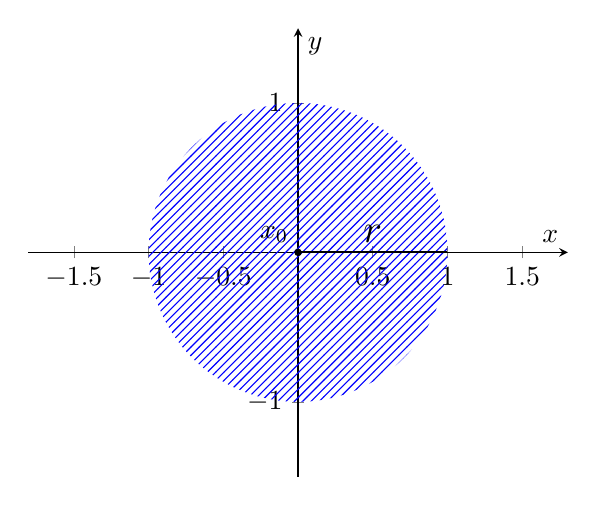
\begin{tikzpicture}
            \begin{axis}[
                axis equal, % Ensures the circle appears round
                axis lines=middle,
                xlabel={$x$},
                ylabel={$y$},
                xmin=-1.5, xmax=1.5,
                ymin=-1.5, ymax=1.5
                ]
                % Plot a circle with radius 1
                \addplot [
                    domain=0:360,       % Angle range
                    samples=200,        % Smoothness
                    fill=none,          % No solid fill color
                    pattern=north east lines, % Hatch pattern
                    pattern color=blue,
                    draw=none           % No outline
                    ] ({cos(x)}, {sin(x)}); 
                \node[above left] (_) at (0, 0){$x_0$};
                \draw[fill=black] (0, 0) circle (0.4mm);
                \draw[thick] (0,0)--(1,0);
                \node[above] (r) at ($(0,0)!0.5!(1,0)$){\Large$r$};
            \end{axis}
        \end{tikzpicture}
        \caption{boules ouverte (i.e $d(x_0, x) < r$)}
    \end{subfigure}
    \hfill
    \centering
    \begin{subfigure}{0.45\textwidth}
        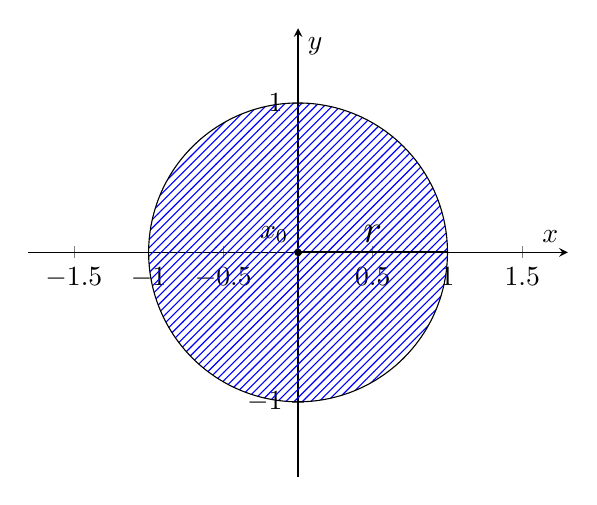
\begin{tikzpicture}
            \begin{axis}[
                axis equal, % Ensures the circle appears round
                axis lines=middle,
                xlabel={$x$},
                ylabel={$y$},
                xmin=-1.5, xmax=1.5,
                ymin=-1.5, ymax=1.5
                ]
                % Plot a circle with radius 1
                \addplot [
                    domain=0:360,       % Angle range
                    samples=200,        % Smoothness
                    fill=none,          % No solid fill color
                    pattern=north east lines, % Hatch pattern
                    pattern color=blue,
                    ] ({cos(x)}, {sin(x)}); 
                \node[above left] (_) at (0, 0){$x_0$};
                \draw[fill=black] (0, 0) circle (0.4mm);
                \draw[thick] (0,0)--(1,0);
                \node[above] (r) at ($(0,0)!0.5!(1,0)$){\Large$r$};
            \end{axis}
        \end{tikzpicture}
        \caption{boules fermée (i.e $d(x_0, x) \le r$)}
    \end{subfigure}
\end{figure}
\begin{lemma}.
   \begin{enumerate}
       \item $B(x_0, 0) = \O$ (car impossible d'avoir des points qui en distance sont strictement plus petit que 0)
       \item $B_f(x_0, 0) = \{x_0\}$
       \item $B(x_0, r_1) \subset B_f(x_0, r_1) \subset B(x_0, r_2)$ si $r_1 < r_2$
       \item\label{lem:lem_boule_4} $B(x_1, r_1) \subset B(x_0, r)$ si  $d(x_0, x_1) + r_1 \le r$
   \end{enumerate} 
   \begin{figure}[H]
       \centering
       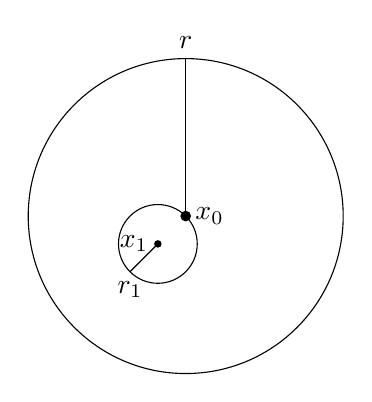
\begin{tikzpicture}
           \coordinate (x_0) at (0,0);
           \def\r{2.0};

           \node[right] (_) at (0, 0){$x_0$};
           \filldraw[color=black] (x_0) circle (0.6mm);
            \node[above] (_) at ($(x_0) + (0, \r)$){$r$};
            \draw (x_0) circle (\r);
            \draw (x_0) -- ($(x_0) + (0, \r)$);

            \def\r_1{0.5};
        \coordinate (x_1) at ($(x_0) - ({\r_1 * cos(45)}, {\r_1 * cos(45)})$);

            \node[left] (_) at (x_1){$x_1$};
            \filldraw[color=black] (x_1) circle (0.4mm);
            \draw (x_1) circle (\r_1);

            \coordinate (x_1r_1) at ($(x_1) - ({ \r_1 * cos(45) }, { \r_1 * cos(45) })$);
            \node[below] (_) at (x_1r_1){$r_1$};
            \draw (x_1) -- (x_1r_1);
       \end{tikzpicture}
       \caption{Lemma ~\ref{lem:lem_boule_4}}
   \end{figure}
\end{lemma}
\begin{explanation}
   Je suppose que $d(x_0, x_1) \le r$\\ 
   Soit $x \in B(x_1, r_1)$ donc $d(x_1, x) < r_1$ à montrer: $x \in B(x_0, r)$ (i.e $d(x_0, x) < r$?)\\
   L'inégalité triangulaire me dit:
   \begin{align*}
       d(x_0, x) &\le d(x_0, x_1) + d(x_1, x)\\
                 &< d(x_0, x_1) + r_1 \le r\\
                 &\implies x \in B(x_0, r)
   \end{align*}
\end{explanation}
\begin{eg}
   \begin{enumerate}
       \item $E = \R$, \quad  $d(x, y) = |x - y|$
            \[
                B(x_0, r) = ]x_0 -r, x_0 + r[
           \] 
       \item $E = \R^d$, \quad $d = 2,3$, \quad $X = (x_1, \ldots, x_d)$ 
           \begin{align*}
               &\|X\|_2 = \left( \sum_{i=1}^{d} x_i^2 \right)^{\frac{1}{2}} \\
               &\|X\|_1 = \sum_{i=1}^{d} x_i\\
               &\|X\|_{\infty} = \underset{1 \le i \le d}{\text{max}}|x_i|
           \end{align*}
           \begin{align*}
              &d_2(X, Y) = \|Y - X\|_2 = \|\vec{XY}\|_2\\ 
              &d_1(X, Y), d_{\infty}(X, Y)
           \end{align*}
   \end{enumerate} 
\end{eg}
\begin{property} Dans $\R^n$
   \begin{itemize}
       \item $d_{\infty}(X, Y) \le d_1(X, Y) \le n d_{\infty}(X, Y)$
       \item $d_{\infty}(X, Y) \le d_2(X, Y) \le \sqrt{n} d_{\infty}(X, Y)$
   \end{itemize} 
\end{property}
\section{Parties bornées de $(E, d)$}
\begin{definition}
    Soit $A \subset E$. $A$ est bornée si  $\exists R > 0$ et $\exists x_0 \in E$ tel que 
    \[
    A \subset B(x_0, R)
    \] 
\end{definition}
\begin{figure}[H]
    \centering
    \incfig{exemple-bornee}
    \caption{Exemple d'un enesemble borné}
    \label{fig:exemple-bornee}
\end{figure}
\begin{lemma}
   Les propriétés suivantes sont équivalentes:
   \begin{enumerate}
       \item $A$ est bornée
       \item  $\forall x_0 \in E, \exists r > 0$ tel que $A \subset B(x_0, r)$
       \item $\exists r > 0$ tel que $\forall x, y \in A$ on a $d(x, y) < r$
   \end{enumerate}
\end{lemma}
\begin{explanation} de lemme
   \begin{itemize}
       \item $(1) \implies (2)$ :\\
           \underline{Hyp}: $\exists x_1 \in E, \exists r_1 \in E$ tq $A \subset B(x_1, r_1)$\\
           Soit $x_0 \in E$. But: trouver $r$ tel que  $A \subset B(x_0, r)$ si $x \in A$, on a:  $d(x_1, x) < r_1$\\
           \underline{Je veux}: $d(x_0, x) <r$\\
          \begin{align*}
              d(x_0, x) \le d(x_0, x_1) + d(x_1, x) \le d(x_0, x_1) + r_1 < r \quad \text{ si } r > d(x_0, x_1) + r_1
          \end{align*} 
   \end{itemize} 
\end{explanation}
\begin{property}
   \begin{enumerate}
       \item Toute partie finie est bornée
       \item Si $A$ bornée et  $B \subset A$ alors $B$ bornée
       \item L'union d'un nombre \underline{fini} de bornés est borné
   \end{enumerate} 
\end{property}
\begin{preuve}{de (3).}\\
    $A_1, \ldots, A_n$ sont bornés. \underline{Je fixe $x_0 \in E$}, $A_i$ borné ($1 \le i \le n$), donc $\exists r_i > 0$ tel que $A_i \subset B(x_0, r_i)$ si $r = \underset{1 \le  i \le n}{max} r_i$ 
    \[
        A_i \subset B(x_0, r), \, \forall i \implies \bigcup\limits_{i=1}^{n} A_i \subset B(x_0, r)
    \] 
\end{preuve}
\section{Fonctions bornées}
\begin{definition}
    Soit $B$ un ensemble. Une fonction  $F: B \to E$ est bornée si $F(B) = \{ F(b): b \in B\} \subset E$ est borné.
\end{definition}
\section{Distance entre ensembles}
\begin{definition}
    La distance entre deux ensembles $A, B$ est:
     \[
         d(A, B) := \underset{x \in A, y \in B}{inf}d(x, y)
    \] 
    Intuitivement, on cherche deux points $x$ et  $y$ tel que la distance est la plus petite possible.
\end{definition}
\begin{definition}
    La distance entre un points $x$ et un ensemble  $B$ est:
     \[
         d(x, B) := \underset{y \in B}{inf}d(x, y)
    \] 
    La même intuition.
\end{definition}
\begin{property}
   $\forall x \in A, \, y \in B, \, d(x, y) \ge d(A, B)$ et $\forall \epsilon > 0, \exists x \in A, \, y \in B$ tq $d(x, y) \le d(A, B) + \epsilon$
\end{property}
\begin{figure}[H]
    \centering
    \incfig{distance-entre-ensembles}
    \caption{Distance entre ensembles}
    \label{fig:distance-entre-ensembles}
\end{figure}
\section{Topologie des espaces métriques}
distance $d(x, y)$ $\longrightarrow$ boules  $B(x_0, r)$ $\longrightarrow$ ensembles ouverts
\begin{definition}
    Soit (E, d) espace métrique.
    \begin{enumerate}
        \item $U \subset E$ est ouvert si $\forall x_0 \in U, \, \exists r > 0 \: r(x_0)$ tel que $B(x_0, r) \subset U$
        \item $F \subset E$ est fermé si $E \setminus F$ est ouvert
    \end{enumerate}
    $\O$ est ouvert et $E$ est ouvert.  $\O$ est fermé et $E$ est fermé.
\end{definition}
\begin{figure}[H]
    \centering
    \begin{subfigure}{0.45\textwidth}
        \centering 
        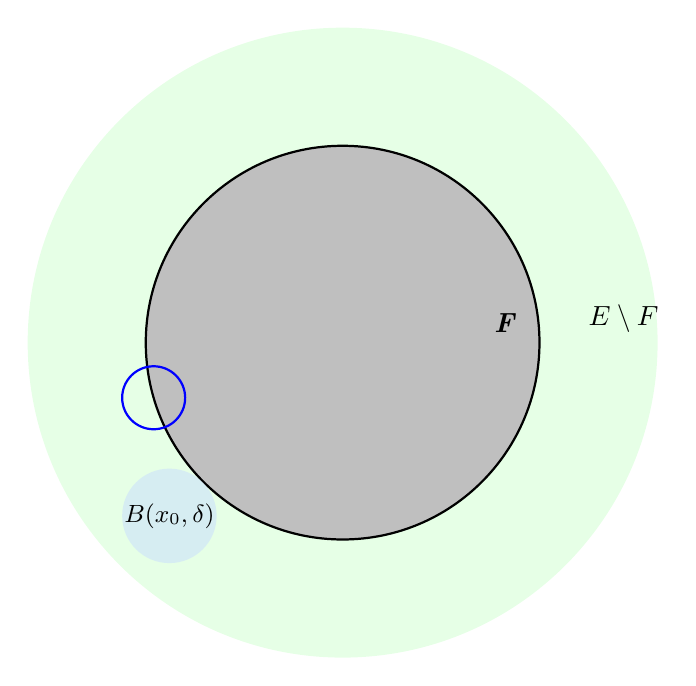
\begin{tikzpicture}
            % Define colors
            \definecolor{lightgreen}{RGB}{230, 255, 230}
            \definecolor{lightblue}{RGB}{200, 220, 255}
            \definecolor{darkgreen}{RGB}{0, 128, 0}

            % Large background circle
            \fill[lightgreen] (0, 0) circle (4cm);

            % Main circle
            \draw[thick, fill=lightgray] (0, 0) circle (2.5cm);
            \node[above right] at (1.8, 0) {\textbf{\textit{F}}};
            \node[above right] at (3, 0) {$E\setminus F$};

            % Small blue circle
            \draw[blue, thick] (-2.4, -.7) circle (0.4cm);

            % Highlighted area for excluded point
            \fill[lightblue, opacity=0.5] (-2.2, -2.2) circle (0.6cm);
            \node (_) at (-2.2, -2.2){\small $B(x_0, \delta)$};
        \end{tikzpicture}
        \caption{Un ensemble fermé\\
            \textit{À la borne, il est impossible de trouver une boules qui appartient à $F$, car il est impossible d'avoir une boule ouverte de  $r = 0$. Exemple: circle bleu foncé}\\
            \textit{Pour tout point dans $E \setminus F$ on peut trouver une boule ouverte}
        }
    \end{subfigure}
    \hfill
    \begin{subfigure}{0.45\textwidth}
        \centering
        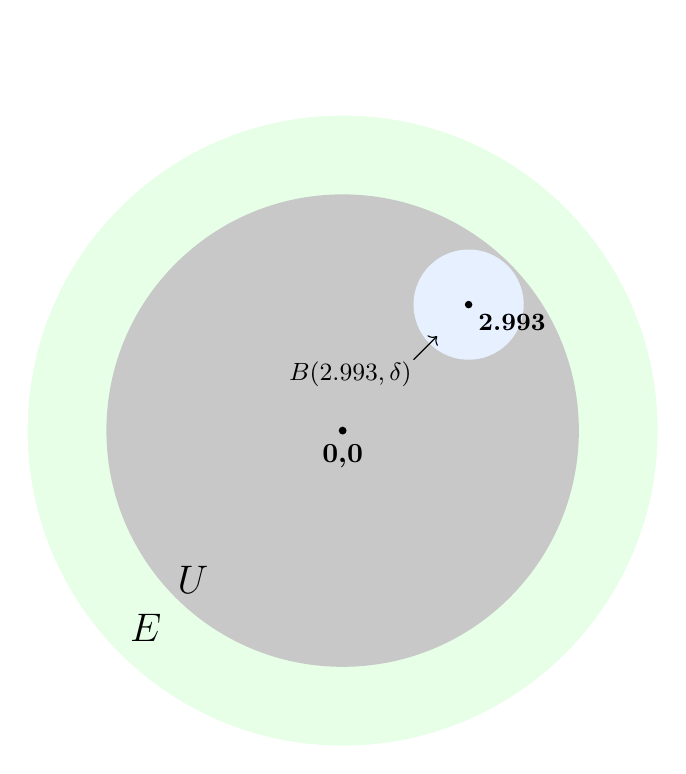
\begin{tikzpicture}
            % Define colors
            \definecolor{lightblue}{RGB}{230, 240, 255}
            \definecolor{lightgray}{RGB}{200, 200, 200}
            \definecolor{darkgreen}{RGB}{0, 128, 0}
            \definecolor{lightgreen}{RGB}{230, 255, 230}

            % Draw large circle
            \fill[lightgreen] (0, 0) circle (4cm);
            \fill[lightgray] (0, 0) circle (3cm);

            % Draw small circle
            \fill[lightblue] (1.6, 1.6) circle (0.7cm);
            \draw[fill=black] (1.6, 1.6) circle(0.4mm);
            \node[below right] at (1.6, 1.6) {\textbf{\small 2.993}};

            \draw[->] (0.9, 0.9)--(1.2, 1.2);
            \node[below left] (_) at (1, 1){\small $B(2.993, \delta)$};
            % Add points and labels
            \node[fill=black, circle, inner sep=1pt, label=below:{\textbf{0,0}}] at (0, 0) {};

            % Add text
            \node[right] at (1, 5) [align=left, text=darkgreen] {
                };
            \node (_) at (-1.9, -1.9){\Large $U$};
            \node (_) at (-2.5, -2.5){\Large $E$};
        \end{tikzpicture} 
        \caption{Un ensemble ouvert\\
            \textit{
                pour tout point pres de la borne
                on peut trouver une boule
                infiniment petite avec des
                points autour ce point inclu dans $U$.
            }
        }

    \end{subfigure}
    \caption{Démonstration des espaces ouverts et fermés}
\end{figure}
\begin{remark}
   dans $\R$ les intervalles ouverts sont des ouverts (pareil pour fermés) 
\end{remark}
\begin{remark}
   Une distance entre deux ensembles ouverts toujours existe et elle est infimum (qui n'est jamais atteint) 
\end{remark}
\begin{lemma}
   \begin{enumerate}
       \item $B(x_0, r_0)$ est ouvert.
       \item $B_f(x_0, r_0)$ est fermé.
   \end{enumerate} 
\end{lemma}
\begin{preuve}
   \begin{enumerate}
       \item Soit $x_1 \in B(x_0, r_0)$ ($d(x_0, x_1) < r_0$).\\
           But: touver $r_1 > 0$ tel que $B(x_1, r_1) \subset B(x_0, r_0)$?\\
           \begin{align*}
               &x \in B(x_1, r_1): \: d(x_1, x) < r_1\\
               &x \in B(x_0, r_0) \text{ si } d(x_0, x) < r_0
           \end{align*}
           facile:
           \begin{align*}
               d(x_0, x) &\le d(x_0, x_1) + d(x_1, x)\\
                         &\le d(x_0, x_1) + r_1\\
                         &< r_0 \text{ si}
           \end{align*}
           $r_1 < r_0 - d(x_0, x_1) > 0$
   \end{enumerate} 
\end{preuve}
\begin{eg} bizzare.\\
    Soit $E = \R$, $d(x, y) = |y - x|$,  $A = ]0, 1[$ ouvert, pas fermé dans  $\R$.\\
    \begin{center}
       \begin{tikzpicture}
          \draw (-2, 0) -- (2, 0); 
          \node (x) at (0, 0){]};
          \node (y) at (1, 0){[};
          \node[below] (x) at (0, -0.2){$0$};
          \node[below] (y) at (1, -0.2){$1$};
          \draw[color=red] (-2, 0) -- (0, 0);
          \draw[color=red] (1, 0) -- (2, 0);
       \end{tikzpicture} 
    \end{center}
    Je regarde $A$ comme partie de  $(A, d)$. Comme  $A \setminus A = \O$ qui est ouvert, donc $A$ est fermé dans $A$. Par contre, les bornes ne sont jamais atteints, alors $A$ est ouvert dans  $(A, d)$.
\end{eg}
\begin{theorem}.
    \begin{enumerate}
        \item Soit $U_i$,  $i \in I$ une collection d'ouverts. Alors,  $\cup_{i \in I} \,U_i$ est ouvert.\\
            Translate: Une union quelconque des ensembles ouverts est ouvert.
        \item Si $U_1, \ldots, U_n$ sont ouverts
            \[
                \bigcap\limits_{i=1}^{n} \, U_i \text{ est ouvert.}
            \] 
            Translate: intersection \underline{finie} des ensembles ouverts est ouvert.
    \end{enumerate}
    \begin{enumerate}
        \item Soit $U_i$,  $i \in I$ une collection de fermés. Alors,  $\cup_{i \in I} \,U_i$ est fermé.\\
            Translate: Une union quelconque des ensembles fermés est fermé.
        \item Si $U_1, \ldots, U_n$ sont fermés 
            \[
                \bigcap\limits_{i=1}^{n} \, U_i \text{ est fermé.}
            \] 
            Translate: intersection \underline{finie} des ensembles fermés est fermé.
    \end{enumerate}
\end{theorem}
\begin{preuve}.
    \begin{enumerate}
        \item Soit $x \in U := \bigcup\limits_{i \in I} U_i$. Il existe un $i$ noté  $i_0$ tel que $x \in U_{i_0}$, $U_{i_0}$ est ouvert, donc $\exists r > 0$ tel que $B(x, r) \subset U_{i_0} \subset U := \bigcup\limits_{i \in I} U_i$.
        \item Soit $x \in U := \bigcap\limits_{1 \le i \le n} U_i$.\\
            On fixe $i$.  $x \in U_i$,  $U_i$ ouvert, donc  $\exists r_i > 0$ tel que $B(x, r) \subset U_i$, $1 \le i \le n$, donc $B(x, r) \subset U := \bigcap\limits_{1 \le i \le n} U_i$
    \end{enumerate}
\end{preuve}

\section{Algorithmes pour montrer qu'un ensemble est ouvert/fermé}
\begin{center}
    
\begin{tabular}{c | c}
    {\large \bf
    Montrer qu'un ensemble est ouvert      } 
 & 
    {\large \bf
    Montrer qu'un ensemble est fermé }
 \\
 \hline
 \parbox[t]{8cm}{
\begin{itemize}
    \item \textbf{Utiliser la définition :} 
    \[
    \forall x \in \mathcal{U}, \exists r > 0 \quad \text{tel que} \quad B(x, r) \subset \mathcal{U}
    \]
    
    \item Montrer que \( E \setminus \mathcal{U} \) est fermé.
    
    \item Montrer que \(\mathcal{U}\) est l'image réciproque d'un ouvert par une application continue.
    
    \item Exprimer \(\mathcal{U}\) comme une boule ouverte.
    
    \item Écrire \(\mathcal{U}\) comme :
    \begin{itemize}
        \item une réunion d'ouverts ;
        \item une intersection finie d'ouverts.
    \end{itemize}
    
    \item \(\mathcal{U} = \operatorname{Int}(U)\).
    
    \item Écrire \(\mathcal{U} = I_1 \times \dots \times I_n\) avec \( I_i \) ouvert.
\end{itemize}
} & \parbox[t]{8cm}{
\begin{itemize}
    \item \textbf{Utiliser la définition :} \( E \setminus V \) est ouvert.
    
    \item \textbf{Caractérisation séquentielle :} Toute suite convergente dans \(V\), sa limite est aussi dans \(V\).
    
    \item Montrer que \(V\) est l'image réciproque d'un fermé par une application continue.
    
    \item Montrer que \(V\) est compact.
\end{itemize}
}
\end{tabular}
\end{center}
\section{Intérieur, adhérent, frontière}
\subsection{Intérieur}
\begin{definition}
    Soit $A \subset E$.
    \begin{enumerate}
        \item $x_0 \in E$ est intérieur à $A$ si  $\exists \, \delta > 0$ tel que:
            \[
            B(x_0, \delta) \subset A
            \] 
        \item $Int(A)$ (intérieur de A) = tous les points intériers à  $A$. (aussi noté $A$)
    \end{enumerate}
\end{definition}
\begin{intuition}
   $Int(A)$ est un ensemble qui se trouve totallement dans $A$ et qui est loin des bords de  $A$.
\end{intuition}
\begin{figure}[ht]
    \centering
    \incfig{interieur-exemple}
    \caption{Exemple d'un intérieur}
    \label{fig:interieur-exemple}
\end{figure}
\begin{prop}
   $Int(A)$ est le plus grand ouvert inclus dans  $A$. De manière équivalente, $Int(A)$ est l'union de tous les ouverts inclus dans  $A$.
\end{prop}
\begin{preuve}
   \begin{enumerate}
       \item $Int(A) \subset A$: clair
       \item \underline{$Int(A)$ est ouvert:} \\
           Soit $x_0 \in Int(A)$. 
           \par
           \textbf{But:} trouver $\delta_0$ tel que  $B(x_0, \delta_0) \subset Int(A)$. Trouver $\delta_0$ tel que si $d(x_0, x) < \delta_0$ alors $x \in Int(A)$ ?
           \par
           \textbf{Hyp:}  $x_0 \in Int(A)$. $\exists \delta_1 > 0$ tel que $B(x_0, \delta_1) \subset A$. On a vu que $B(x_0, \delta_1)$ est ouvert.
           Je dis que $B(x_0, \delta_1) \subset Int(A)$.
           \par
           \textbf{Preuve}: Soit $x \in B(x_0, \delta_1)$. $B(x_0, \delta_1)$ ouvert, donc $\exists \delta_2 > 0$ tel que $B(x, \delta_2) \subset B(x_0, \delta_1) \subset A$. Donc $x \in Int(A)$, donc  $B(x_0, \delta_1) \subset Int(A)$.\par
           $Int(A)$ est ouvert.
       \item Si $U$ est ouvert et  $U \subset A$ alors $U \subset Int(A)$?
           \par
           $x_0 \in U$. $U$ ouvert  $\implies$ $\exists \delta$ tel que $B(x_0, \delta) \subset U \subset A$ $\implies$ $x_0 \in Int(A)$
   \end{enumerate} 
\end{preuve}

\subsection{Adhérent}
\begin{definition}
    Soit $A \subset E$. 
    \begin{enumerate}
        \item $x_0 \in E$ est \underline{adhérent} à $A$, si  $\forall \delta > 0, \, B(x_0, \delta)$ intérsecte $A$. (équivalent à $d(x_0, A) = 0$)
        \item $Adh(A)$ (adhérence ou fermeture de $A$) = ensemble des points adhérents à $A$ (aussi noté $\overline{A}$)
    \end{enumerate}
\end{definition}
\begin{intuition}
   Adherent aide à completer des ensembles. Si $A$ est ouvert, alors ses bords n'appartiennent pas à  $A$, mais ils appartiennent à  $Adh(A)$ .
\end{intuition}
\begin{figure}[H]
   \centering 
    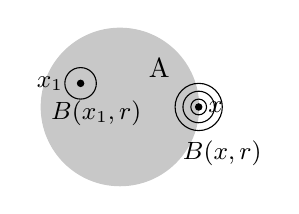
\begin{tikzpicture}
            \definecolor{lightgray}{RGB}{200, 200, 200}
        \filldraw[color=lightgray] (0,0) circle (1cm); 
        \coordinate (x) at (1, 0);
        \filldraw[color=black] (x) circle (0.4mm);
        \node[right] (_) at (x){\small $x$};
        \node (_) at (0.5, 0.5){A};

        \draw (x) circle (0.2cm);
        \draw (x) circle (0.3cm);
        \draw (x) circle (0.1cm);
        \node[below] (_) at (1.3, -0.3){\small $B(x, r)$};

        \draw (-0.5, 0.3) circle (0.2cm);
        \filldraw[color=black] (-0.5, 0.3) circle (0.4mm);
        \node[left](_) at (-0.6, 0.3){\small $x_1$};
        \node[below] (_) at (-0.3, 0.2){\small $B(x_1, r)$};
    \end{tikzpicture} 
    \caption{Adhérent}
\end{figure}
\begin{prop}
   $Adh(A)$ est le plus petit fermé qui contient $A$ (l'intérsection de tous les fermés qui contiennent $A$)
\end{prop}
\begin{preuve}
   \begin{enumerate}
       \item $A \subset Adh(A)$ clair
       \item $Adh(A)$ est fermé?
           \par On montre que  $E \setminus Adh(A)$ est ouvert. \par 
           $x_0 \in Adh(A)$ $\iff$ $\forall \delta > 0, \, B(x_0, \delta) \cap A \neq \O$ \par
           $x_0 \not\in Adh(A)$ $\iff$ $\exists \delta_0 > 0$ tq $B(x_0, \delta_0) \cap A = \O$ $\iff$ $\exists \delta_0>0$ tq $B(x_0, \delta_0) \subset E\setminus A$ $\iff$ $x_0 \in Int(E\setminus A)$ 
           \par Alors:
           \begin{align*}
               &E \setminus Adh(A) = Int(E \setminus A)\\
               &Adh(A) = (Int(\underbrace{A^{c}}_{= E \setminus A}))^{c}
           \end{align*}
   \end{enumerate} 
\end{preuve}
\begin{definition}
    Soit $A \subset B$. On dit que $A$ est \textbf{dense} dans  $B$ si  $B \subset Adh(A)$
    \par
    Soit $x_0 \in B, \, \forall \epsilon > 0 \, \exists  x_{\epsilon} \in A$ tel que $d(x_0, x_{\epsilon}) < \epsilon$
\end{definition}
\begin{eg}
   \[
       \Q^2 = \{(x, y): x,y \in \Q\} \text{ dense dans } \R^2
   \]  
   
\end{eg}
\begin{definition}
    alternative de densité. Soit $A \subset B$. $A$ est dense dans  $B$ si toute boule ouverte de  $B$ contient au moins un élémens de  $A$.
\end{definition}

\subsection{Frontière}
 \begin{definition}
     Soit $A \subset E$. La \textbf{frontière} de $A$ (ou le bord de $A$) noté $Fr(A)$ ou  $\partial A$ c'est:
      \[
     Adh(A) \cap Adh(E \setminus A)
     \] 
 \end{definition}
 \begin{eg} dans $\R$
    \begin{enumerate}
        \item $Int(\Q) = \O$
        \item $Int(\R \setminus \Q) = \O$
        \item $Adh(\Q) = \R$
        \item $Adh(\R \setminus \Q) = \R$
        \item $Fr(\Q) = \R$
        \item $Fr(\R \setminus \Q) = \R$
    \end{enumerate} 
 \end{eg}
 \begin{eg} $E = \{a, b, c\}$
    On pose:
    \begin{itemize}
        \item $d(a,a) = d(b,b) = d(c,c) = 0$
        \item  $d(a,b) = d(b,a) = d(b,c) = d(b,c) = 1$
        \item  $d(a,c) = d(c, a) = 2$
    \end{itemize}
    \[
        B(a,2) = \{a, b\} = Adh(B(a, 2))
    \] 
    \[
        B_f(a, 2) = \{a, b, c\}
    \] 
 \end{eg}
 \begin{prop}
    \begin{enumerate}
        \item $Int(A) \subset A \subset Adh(A)$
        \item $E = Int(E \setminus A) \cup Fr(A) \cup Int(A)$ (union disjointe)
        \item $E \setminus Int(A) = Adh(E \setminus A)$
        \item $E \setminus Adh(A) = Int(E \setminus A)$
        \item $Fr(A) = Adh(A) \setminus Int(A)$
    \end{enumerate} 
 \end{prop}
 \begin{prop}
     \begin{enumerate}
         \item $A$ ouvert  $\iff$ $A = Int(A)$
         \item  $A$ fermé  $\iff$ $A = Adh(A)$
         \item  $x \in Adh(A)$  $\iff$ $d(x, A) = 0$
         \item  $x \in Int(A)$  $\iff$ $d(x, E \setminus A) > 0$
     \end{enumerate}
 \end{prop}

 \section{Suite dans un éspace métrique}
 \begin{definition}
     $E$ un ensemble. Une suite dans $E$: notée $(u_n)_{n \in \N}$ c'est une fonction $u:  \N \to E$ où $u(n)$ est noté  $u_n$ est le le  $\text{n}^{\text{ième}}$ terme de la suite $(u_n)_{n \in \N}$.
     \par
     Si $E = \R^d$
     \[
     \R^d \ni X_n = (x_{1,n}, \ldots, x_{d,n})
     \] 
 où $(x_{i,n})_{n \in \N}$ suites dans $\R$
 \end{definition}
 \begin{definition}
     Soit $(x_n)$ une suite dans  $E$ et  $x \in E$. On dit que  $\lim_{n \to \infty} x_n = x$ si $\lim_{n \to \infty} d(x_n, x) = 0$.
     \par
     ($\forall \epsilon > 0, \, \exists N \in \N \, \text{ tq si } n \ge N, \, d(x_n, x) < \epsilon$)
 \end{definition}
 \begin{prop}
     $(x_n)_{n \in \N}$ est bornée si $\{x_n : n \in \N\} (\subset E)$ est un ensemble borné. 
 \end{prop}
 \begin{remark}
    dans $\R^d$ muni de $d_2$ (distance euclidienne)

    \begin{align*}
        &X_n = (x_{1,n}, \ldots, x_{d,n})\\
        &X = (x_1, \ldots, x_d)
    \end{align*}
    \[
    \lim_{n \to \infty} X_n = X \iff \lim_{n \to \infty} x_{i,n} = x_i \quad (1 \le i \le d)
    \] 
 \end{remark}
 \begin{prop}
    la limite d'une suite convergente est unique. 
 \end{prop}
 \begin{preuve}
    \[
    \text{Si } X_n \xrightarrow[n \to \infty]{} X \text{ et } X_n \xrightarrow[n \to \infty]{} X'
    \]  
    \[
        d(X, X') \le \underbrace{d(X, X_n)}_{\to 0} + \underbrace{d(X_n, X')}_{\to 0} \implies d(X, X') = 0 \implies X = X'
    \] 
 \end{preuve}
 \begin{prop}\label{prop:suite-lien-avec-adherence}
     (lien aven l'adhérence) 
     \begin{enumerate}
         \item $x \in Adh(A)$ si et seulement s'il existe une suite  $(x_n)$ d'éléments de  $A$ telle que  $\lim_{n \to \infty} x_n = x$
         \item $A$ est fermé ssi pour toute suite  $(x_n)$ d'éléments de  $A$ qui converge vers $x \in E$ on a $x \in A$
     \end{enumerate}
 \end{prop}
\begin{intuition}
   \begin{enumerate}
       \item Si $(x_n)_{n \in \N}$ est d'éléments de  $A$ ($\forall n \in N, \, x_n \in A$), donc elle converge vers un éléments $x$ qui peut être soit dans  $A$, soit à la borne des éléments de  $A$, alors à la frontière. 
       \item Si la limite de toute suite $(x_n)_{n \in \N}$ des éléments de  $A$ est aussi dans  $A$, alors la frontière de  $A$ est inclu dans  $A$. Car l'une des suites tend vers la borne.
   \end{enumerate} 
\end{intuition}
\begin{preuve} de Prop. \ref{prop:suite-lien-avec-adherence}
    \begin{enumerate}
        \item ($\impliedby$) Soit $(x_n)$ avec  $x_n \in A \quad \forall n \in \N$ et $\lim_{n \to \infty} x_n = x$.
            \par
            J'ai $d(x_n, x) \xrightarrow[n \to \infty]{} 0$ et $x_n \in A$, donc
             \[
                 inf_{y \in A}(d(x, y)) = 0 = d(x, A)
            \] 
            \[
            d(x, A) = 0 \iff x \in Adh(A)
            \] 
            \par
            ($\implies$) Soit $x \in Adh(A)$
             \begin{align*}
                 \iff& d(x, A) = 0\\
                \iff& \forall \epsilon > 0, \, \exists x_{\epsilon} \in A \text{ tel que } d(x, x_{\epsilon}) < \epsilon
            \end{align*}
            Prendre $\epsilon = \frac{1}{n}$, je pose $u_n = x_{\frac{1}{n}}$. $u_n \in A$  $d(x, u_n) < \frac{1}{n}$, donc $\lim_{n \to \infty} u_n = x$ 
        \item ($\implies$) Soit $A$ fermé, donc 
             \[
            A = Adh(A)
            \] 
            Si $(x_n)$ suite dans  $A$ qui converge vers  $x$.
             \[
            x \in Adh(A) = A
            \] 
            ($\impliedby$) On dit que $Adh(A) \subset A$. Comme $A \subset Adh(A)$, donc $A = Adh(A)$
    \end{enumerate} 
 \end{preuve}
\section{Suites de Cauchy}
\begin{definition}
    $(x_n)_{n \in \N}$ suite dans $E$ est de \underline{Cauchy} si:
     \[
    \forall \epsilon > 0 \, \exists N(\epsilon) \in \N \text{ tel que } \forall n, p \ge N(\epsilon), d(x_n, x_p) \le \epsilon
    \] 
\end{definition}
\begin{intuition}
   Une suite de Cauchy c'est comme on mesure un point et on le localise, i.e:
   \begin{enumerate}
       \item On dit qu'il est entre $0$ et  $1$.
       \item Ensuite, on precise plus et on dit qu'il est entre  $0.5$ et  $0.6$.
       \item Puis, entre  $0.55$ et  $0.56$
   \end{enumerate}
   On peut infiniment augmenter le niveau de précision. C'est ça l'idée d'une suite de Cauchy.
\end{intuition}
\begin{prop}
   \begin{enumerate}
       \item Toute suite de Cauchy est bornée.
        \item Toute suite convergente est de Cauchy
   \end{enumerate} 
\end{prop}
\begin{preuve}
   \begin{enumerate}
       \item Soit $(x_n)_{n \in \N}$ une suite de Cauchy. Alors, par définition
           \[
           \forall \varepsilon > 0, \, \exists N \in \N \text{ tq } \forall n, p \ge N, d(x_n, x_p) < \varepsilon
           \] 
           Soit $\varepsilon = 1$. Donc  $\exists N \in \N$ tq $\forall n, p \ge N, d(x_n, x_p) < 1$, donc $\forall n \ge N$, $d(x_n, x_N) < 1$. On a donc:
           \[
               \forall n \in  N, d(x_n, x_N) < 1 + \overbrace{\sup_{1 \le i \le N}d(x_n, x_N)}^{=: r_0}
           \] 
           Alors $\forall n \in \N, \, x_n \in B(x_N, 1 + r_0)$ donc $(x_n)_{n \in \N}$ bornée.
       \item Soit $(x_n)$ une suite avec  $\lim_{n \to \infty} x_n = x$ avec $x \in E$.
           \begin{itemize}
               \item 
                   \underline{Hyp:}  $\frac{\epsilon}{2} > 0 \, \exists N(\frac{\epsilon}{2}) \in \N \text{ tel que } \forall n \ge N(\frac{\epsilon}{2}), d(x_n, x) \le \epsilon/2$
                \item 
                    \underline{À montrer:} $\epsilon > 0 \, \exists M(\epsilon) \in \N \text{ tel que } \forall n, p \ge M(\epsilon), d(x_n, x_p) \le \epsilon$
           \end{itemize}
           \[
               d(x_n, x_p) < d(x_n, x) + d(x, x_p) \text{ si } n, p \ge  N(\frac{\epsilon}{2}) \, d(x_n, x_p) \le 2 \frac{\epsilon}{2} = \epsilon
           \] 
   \end{enumerate} 
\end{preuve}
\begin{definition}
    $(E, d)$ est \underline{complet} si toute suite de cauchy dans  $E$ est convergente.
\end{definition}
\begin{definition}
    Un éspace métrique $(E, d)$ est \textbf{complet} si toute suite  $(x_n)_{n \in \N}$ d'éléments de  $E$ converge vers une limite  $x$ qui appartient aussi à  $E$.
\end{definition}
\begin{intuition}
   Ce n'est pas très correcte à dire, mais, on peut dire qu'une suite de Cauchy $(x_n)_{n \in \N}$ converge toujours car il existe un moment $N \in \N$ après lequel les éléments sont très proches mais la limite n'appartient pas toujours à l'ensemble dans lequel cette suite est de Cauchy. 

   Par exemple, une suite $(u_n)_{n \in \N}$ à valeur dans $\Q$ qui converge vers $\sqrt{2} $ dans $\R$. Dans $\R$ elle est convergente et de Cauchy, mais dans $\Q$ elle est de Cauchy mais \underline{pas convergente} car la limite $\sqrt{2} \not\in \Q $.
\end{intuition}
\begin{eg}
    Un éspace métrique $(]0, 1], d)$ avec $d$ une distance euclidienne n'est pas complet, car  soit une suite: $x_n = \frac{1}{n}$ dont la limite est $0$. Par contre,  $0 \not\in ]0, 1]$. Donc cet éspace n'est pas complet. 
\end{eg}
\begin{figure}[h]
   \centering 
   \begin{tikzpicture}
       \draw[->] (-1, 0) -- (2, 0); 
       \node[below] (_) at (2,0){$x$};

       \node (_) at (0,0){]};
       \node[below] (_) at (0,-0.3){$0$};
       \node (_) at (1,0){]};
       \node[below] (_) at (1,-0.3){$1$};
       \draw[color=red] (0,0)--(1,0);
   \end{tikzpicture}
   \caption{$(]0, 1], d)$ n'est pas complet}
\end{figure}
\begin{eg}
   Un éspace $(\Q, d)$ n'est pas complet. Car on peut prendre une suite  $x_n$ tendant vers  $\sqrt{2} \not\in \Q$.
\end{eg}

\begin{figure}[H]
    \centering
    \incfig{q_not_complete}
    \caption{$\Q$ pas complet}
    \label{fig:q_not_complete}
\end{figure}
\begin{prop}\label{prop:rd-est-complet}
   $\R^d$ muni de la distance usuelle est complet. 
\end{prop}
\begin{preuve}
   \[
   X_n = (x_{1,n}, \ldots, x_{d,n})
   \]  
   \[
   |x_i - y_i| \le d(X, Y) = \|X - Y\|_2 \quad \forall 1 \le i \le d
   \] 
   les suites réelles $(x_{i,n})_{n \in \N}$ sont de Cauchy si $(X_n)$ est de Cauchy.
\end{preuve}
\begin{property}
   $\R$ est complet 
\end{property}
\begin{preuve}
    (Suit de la propriété de la borne supérieure) 
    \par
    Il existe $x_i \in \R$ avec $1 \le i \le d$ tels que $|x_{i,n} - x_{i}| \xrightarrow[n \to \infty]{} 0$
    \[
        d(X, Y) \le \sqrt{d} \underset{1 \le i \le d}{max} |x_i - y_i| 
    \] 
    donc $X_n \xrightarrow[n \to \infty]{} X$, $X = (x_1, \ldots, x_d)$
\end{preuve}
\section{Sous-suites}
\begin{definition}
    Soit $(x_n)_{n \in \N}$ une suite dans $E$. Une suite  
    \[
        (y_n)_{n \in \N} \text{ avec } y_n = x_{\phi(n)}
    \] 
    où $\phi: \N \to \N$ est \underline{strictement croissante} est appelée \textbf{sous-suite} de la suite $(x_n)$.
\end{definition}
\begin{eg}
    Soit une application $\phi: \N \to \N$ telle que $\phi(n) = 2n$. Donc  $(x_n)_{\phi(n)}$ est une sous-suite de  $(x_n)_{n \in \N}$ et:
    \[
        (x_n)_{\phi(n)} = \{x_0, x_2, x_4, \ldots\}
    \] 
\end{eg}
\begin{prop}
   \begin{enumerate}
       \item Toute sous-suite d'une suite convergente converge vers la limite de cette suite.
           \par
           Cela signifie que, $\forall (x_n)_{n \in \N}$ tq $\exists x \in E, \lim_{n \to \infty} x_n = x$
           \[
               \forall \phi: \N \to \N \text{ strictement croissante}, \lim_{n \to \infty} x_{\phi(n)} = x
           \] 
        \item Si $(x_n)$ est de Cauchy et admet une sous-suite qui converge vers  $X$, alors  $(x_n)$ converge vers  $x$.
   \end{enumerate} 
\end{prop}
\begin{preuve}
   \begin{enumerate}
       \item Soit $(x_n)$ avec  $\lim x_n = x$
            \[
                \forall \epsilon > 0 \, \exists M(\epsilon) \text{ tq si } n \ge N(\epsilon), d(x_n ,x) \le \epsilon 
           \] 
           Soit $y_n = x_{\phi(n)}$ une sous-suite.
           \begin{itemize}
               \item \underline{But:} Soit $\epsilon > 0$, trouver $N(\epsilon)$ tq si  $n \ge  N(\epsilon), \, d(\underbrace{y_n}_{:= x_{\phi(n)}}, x) \le \epsilon$
           \end{itemize}
           Je choisis $N(\epsilon)$ tel que si  $n \ge N(\epsilon)$ alors $\phi(n) \ge M(\epsilon)$, donc $d(y_n, x) d(x_{\phi(n)}, x) \le  \epsilon$. C'est possible car $\phi(n) \xrightarrow[n \to \infty]{} \infty$, $N(\epsilon) = M(\epsilon)$ 
        \item 
            \begin{itemize}
                \item  \underline{Hyp1:} $\forall \epsilon > 0 \, \exists M(\epsilon)$ tq si $n, p \ge M(\epsilon)$ $d(x_n, x_p) \le \epsilon$
                \item  \underline{Hyp2:} $\forall \epsilon > 0 \, \exists P(\epsilon)$ tq si $p \ge P(\epsilon), d(y_p, x) \le \epsilon$, $d(y_p, x) = d(x_{\phi(p)}, x)$
            \end{itemize}
            \begin{align*}
                d(x_n, x) \le d(x_n, x_{\phi(p)}) + d(x_{\phi(p)}, x) \quad \text{par l'inégalité triangulaire}
            \end{align*}
            \begin{align*}
                d(x_n, x_{\phi(p)}) \le \epsilon \text{ si } n \ge M(\epsilon) \text{ et } \phi(p) \ge M(\epsilon)
            \end{align*}
            \begin{align*}
                d(x_{\phi(p)}, x) \le \epsilon \text{ si } p \ge P(\epsilon)
            \end{align*}
            Si $n \ge M(\epsilon)$, je choisis $p$ tel que  $\phi(p) \ge  M(\epsilon)$ et $p \ge P(\epsilon)$. Je fixe ce $p$!
             \[
            \text{si } n \ge M(\epsilon) \text{ alors } d(x_n, x) \le 2\epsilon
            \] 
   \end{enumerate} 
\end{preuve}

\section{Procédé de construction de l'intérieur et l'adhérence}
J'ai $A \subset \R$ ou $\R^2$ (ou $\R^3$). Je dois trouver $Int(A)$ et  $Adh(A)$
 \begin{enumerate}
    \item Je dessine $A$ sur une feuille
    \item Je pense que  $Int(A) = C$ ($C$ dit être inclu dans  $A$!)
         \begin{enumerate}
             \item Je montre que \underline{$C$ est ouvert} (facile), donc
                 \[
                 C \subset Int(A)
                 \] 
                 car $Int(A)$ est le plus grand ouvert inclu dans  $A$.
            \item Je montre que $Int(A) \subset C$, i.e je montre que les points dans $A$ mais pas dans  $C$ ne sont pas dans  $Int(A)$: je prends $X \in A, X \not\in C$, je montre que $X \not\in Int(A)$
                Je construit une suite $(X_n)$ avec  $X_n \not\in A$ mais  $X_n \to X$.
         \end{enumerate}
    \item Je pense que $Adh(A) = B$ (il faut que $A \subset B$)
        \begin{enumerate}
            \item Je montre que $B$ est fermé (facile)
                \[
                \text{donc } Adh(A) \subset B
                \] 
            \item  On montre que $B \subset Adh(A)$: On fixe $X \in B$, on cherche une suite  $(X_n)$ avec  $X_n \in A$ et  $X_n \xrightarrow[n \to \infty]{} X$. 
                \underline{On regarde seulement les} $X \in B, X \not\in A$
        \end{enumerate}
\end{enumerate}
\begin{eg}
   \[
       A = \{(x, y) \in \R^2 \mid 2x + 3y \le 4, x \neq y\}
   \]  
\begin{figure}[H]
    \centering
    \incfig{example-interieur}
    \caption{Exemple de l'intérieur}
    \label{fig:example-interieur}
\end{figure}
.
\begin{itemize}
    \item 
        Je dévine que $Int(A) = C = \{(x, y) \mid 2x + 3y < 4, x \neq y\}$
    \item
        Convect: $\{(x, y) \mid 2x + 3y < 4, x < y\} \cup \{(x, y) \mid 2x + 3y < 4, x > y\}$
\end{itemize}
Je construit une suite $(X_n)$ avec  $X_n \not\in A$ mais $X_n \to X$. Soit $X \in A, X \not\in C$, $X = (x, y)$ donc:  $2x + 3y = 4 \quad x \neq y$
\[
X_n = (x, y + \frac{1}{n})
\] 
\[
2x_n + 3y_n = 2x + 3y + \frac{3}{n} = 4 + \frac{3}{n} > 4
\] 
\[
X_n \not\in A \text{ mais } X_n \to X
\] 
\end{eg}
\begin{eg}
   \[
       A = \{(x, y) \in \R^2 \mid x > 0, y = x^{-1}\}
   \]  
   $Int(A) = \O$? $C = \O$
\begin{figure}[H]
    \centering
    \incfig{example-interieur-hyperbola}
    \caption{Exemple de l'intérieur de l'hyperbole}
    \label{fig:example-interieur-hyperbola}
\end{figure}
$\O$ ouvert, donc $C \subset Int(A)$
\par
Soit $X \in A \quad X \not\in C$, donc $X \in A$.
 \[
X_n := (x, y + \frac{1}{n}) \quad X_n \not\in A
\] 
\[
x_ny_n = xy + \frac{x}{n} = 1 + \frac{x}{n} \neq 1
\] 
\[
X_n \xrightarrow[n \to \infty]{} X \text{ donc } X \not\in Int(A)
\] 
\[
Int(A) = \O
\] 
\end{eg}
\begin{eg}
   \[
       A = \{(x, y) \in \R^2 \mid x > 0, y = x^{-1}\}
   \]  
   $Adh(A) = ?$
   \par
   Je pense que  $Adh(A) = A$ ($B = A$). Il suffit de montrer que $A$ \underline{est fermé}.
    \[
   x > 0 \quad y \le \frac{1}{x} \quad y \ge \frac{1}{x}
   \] 
   Si $X_n = (x_n, y_n)$  \quad $X_n \in A$ et  $X_n \to X$, alors $X \in A$
    \[
        X = (x, y) \quad \substack{x_n \to x \\ y_n \to y} \quad \substack{x_n \to x \\ \frac{1}{x_n} \to y} \quad (x_n > 0)
   \] 
   donc $x > 0$ et  $y = \frac{1}{x}$ donc $X \in A$
    \[
   A \text{ est fermé}
   \] 
\end{eg}
\begin{eg}
   \[
       A = \{(x, y) \in \R^2 \mid 2x + 3y \le 4, x \neq y\}
   \]  
\begin{figure}[H]
    \centering
    \incfig{example-adherence}
    \caption{example-adherence}
    \label{fig:example-adherence}
\end{figure}
.
\begin{enumerate}
    \item 
        $B$ est fermé (facile), donc  $Adh(A) \subset B$
    \item Soit $X \in B$. On montre que  $X \in Adh(A)$ (on cherche $X_n \in A$ avec  $X_n \to X$) 
        \par
        Je regarde juste $X \in B, X \not\in A$
        \[
        X_n = (x_n, y_n) \in A \quad x_n \to x \text{ et } y_n \to y
        \] 
        \[
        x_n = x + \frac{1}{n}, y_n = y = x
        \] 
        \[
        X_n \to X \text{ et } 2x_n + 3y_n = 2x + 3y - \frac{2}{n} \le 4 et x_n \neq y_n 
        \] 
        donc $X_n \in A$
\end{enumerate}
\end{eg}
\begin{eg}
   \[
       A = \{(x, y) \mid |x| \le 1, |y| < 1\}
   \]  
   \[
       Int(A) = \{(x, y) \mid |x| < 1, |y| < 1 \}
   \] 
   \[
       Adh(A) = \{(x, y) \mid |x| \le 1, |y| \le 1\}
   \] 
\end{eg}
\begin{eg}
   \[
       A = \{(x,y) \mid x > 0, y = \sin(\frac{1}{n}) \}
   \]  
   $Adh(A) = A \cup \{(0, y) \mid -1 \le y \le 1\}$
   $Int(A) = $
\end{eg}
\section{Compacité}
\begin{definition}
   Soit $F \subset E$. Un recouvrement ouvert de $F$ est une collection  $(U_i)_{i \in I}$ où $U_i$ sont des ouverts et $F \subset \cup_{i \in I} U_i$ ("les $U_i$ recouvrent  $F$")
\end{definition}
\begin{eg}
\begin{figure}[H]
    \centering
    \incfig{recouvrement-ouvert}
    \caption{recouvrement-ouvert}
    \label{fig:recouvrement-ouvert}
\end{figure}
\begin{itemize}
    \item $U_x = B(x, \frac{1}{2})$
    \item $\bigcup_{x \in F} U_x$ contient $F$
    \item  $(U_x)_{x \in F}$ recouvrement ouvert de $F$
\end{itemize}
\end{eg}

\begin{definition}
    $K \subset E$ est compact si de tout recouvrement ouvert $(U_i)_{i \in I}$ de $F$ on peut extraire un sous-recouvrement fini: je peux choisir  $i_1, \ldots, i_n \in I$ tels que 
    \[
    F \subset U_{i_1} \cup U_{i_2} \cup \ldots \cup U_{i_n}
    \] 
\end{definition}
\begin{property}
   Un ensemble fini est compact. 
   \[
       F = \{a_1, \ldots, a_p\} \quad a_j \in E
   \] 
   $(U_i)_{i \in I}$ recouvre $F$.
   Je choisit  $a_j$ (point de $F$), il existe un $i \in I$ noté  $i(j)$ tel que 
    \[
   a_j \in U_{i(j)} \quad F \subset U_{i(1)} \cup \ldots \cup U_{i(p)}
   \] 
\end{property}
\begin{theorem}
    Caractérisation à l'aide de suites. \par
    $K \subset E$ est compact ssi toute suite d'éléments de $K$ admet une sous-suite qui converge vers un élément de  $K$.
\end{theorem}
\begin{eg}
    \begin{figure}[H]
        \centering
        \incfig{compactness-with-sequences}
        \caption{compactness-with-sequences}
        \label{fig:compactness-with-sequences}
    \end{figure}
    \begin{itemize}
        \item $E = \R^2$
        \item $F = B(x_0, r)$ pas compact
        \item $x_n \in F$,  $x_n \to x$, $x \not\in F$
        \item si $y_n = x_{\phi(n)}$, $y_n \to x$ mais $x \not\in F$
    \end{itemize}
\end{eg}
\begin{eg}
    
\begin{figure}[H]
    \centering
    \incfig{suite-sans-sous-suite-convergente}
    \caption{suite-sans-sous-suite-convergente}
    \label{fig:suite-sans-sous-suite-convergente}
\end{figure}
\[
    F = \{(x, y): x \ge 0, -\frac{1}{x} \le y \le \frac{1}{x} \}
\] 
$u_n = (n, 0)$  $(u_n)$ suite dans  $F$ sans sous-suite convergente.
\end{eg}

\begin{prop}
    \begin{enumerate}
        \item $K$ compact $\implies$ $K$ fermé et borné. (réciproque est fausse en général!)
        \item Si $K$ compact et $F$ fermé, alors  $K \cap F$ est compact.
        \item Si $K$ compact, toute suite de Cauchy dans  $K$ converge dans  $K$
    \end{enumerate}
\end{prop}

\begin{preuve}
   \begin{enumerate}
       \item Soit $K$ compact.  $K$ fermé si  $(u_n)$ suite dans  $K$ qui converge vers  $u$, alors  $u \in K$.
           \par
           \underline{clair:}  $(u_n)$ a une suite-suite  $v_n = u_{\phi(n)}$ avec $v_n \to v \in K$, $u_n \to u$, donc $v_n \to u$ $\implies$ $u = v$  $\implies$ $u \in K$
           \par
           $K$ \underline{est borné}:
           \par
              Soit $U_x = \bigcup_{x \in K} B(x, 1)$ un recouvrement ouvert de $K$. Or  $K$ est compact, donc il existent  $x_1, \ldots, x_n \in K$, tels que $K \subset \bigcup_{i = 1, \ldots, n} B(x_i, 1) $, donc $K$ est borné.
        \item $K$ compact et $F$ fermé. $(u_n)$ une suite dans $K \cap F$. $u_n \in K$. $ \exists$ sous-suite $v_n = u_{\phi(n)}$ avec $v_n \to x \in K$. $v_n \in F, v_n \to x$, $F$ fermé donc $x \in F$, $x \in K \cap F$.
        \item Soit $(u_n)$ suite de Cauchy dans $K$. $(u_n)$ a une sous-suite $v_n = u_ { \phi(n)}$ qui converge vers $x \in K$. $u_n \to x \in K$
   \end{enumerate} 
\end{preuve}

\subsection{Compacité dans $\R^n$ avec la distance usuelle}
\begin{theorem}
    (Borel-Lebesgue)
    \par
    dans $\R^n$ avec la distance usuelle $K$ est compact ssi  $K$ est fermé et borné
\end{theorem}

\begin{prop}\label{prop:boules-fermes-sont-compactes}
   Les boules fermées $B_f(x_0, r)$ sont compactes dans $\R^n$. 
\end{prop}
\begin{itemize}
    \item Implique le théorème: Soit $K$ fermé et borné.  $K$ borné, donc  $K \subset B_f(0, r)$ avec $r$ grand, donc  $K = K \cap B_f(0, r)$. Donc  $K$ compact.
\end{itemize}
\begin{preuve} de la prop. \ref{prop:boules-fermes-sont-compactes}
   \begin{enumerate}
       \item $n = 1$.  À montrer: $[a, b]$ est compact.
           \par
           Soit  $(U_i)_{i \in I}$ un recouvrement ouvert de $[a, b]$. Soit  $F$: les  $x \in [a, b]$ tels que  $[a, x]$ est récouvert par un nombre fini de  $U_i$.
           \par
           \underline{But:} montrer que  $b \in F$! (si $x \in F$, et  $x' \le x$ $x' \in F$)
            \begin{enumerate}
                \item $F \neq \O$: $a \in F$  $[a, a] = \{ a \}$
                \item  $c = sup(F)$. \underline{On montre que $c = b$} \par
                    Supposons que $c < b$.
                     \begin{itemize}
                        \item $c$ appartient à un des  $U_i$ noté  $U_{i_0}$
                        \item $U_{i_0}$ est ouvert, $c \in U_{i_0}$ donc $\exists \delta_0 > 0$ tel que $]c - \delta_0, c + \delta_0[ \subset U_{i_0}$
                        \item $c = sup(F)$:  $\forall \delta > 0, \, \exists x_{\delta} \in F$ avec $c - \delta < x_{\delta} \le c$
                            \[
                            \delta = \delta_{0,2} \quad \exists x_{\delta_0} \in F, c - \delta_{0,2} < x_{\delta_0}
                            \] 
                            $[a, x_{\delta_0}]$ reouvert par $U_{i_1} \cup \ldots \cup U_{i_n}$ et $]c - \delta_0, c + \delta_0[ \subset U_{i_0}$ donc $[a, c + \delta_{0,2}]$ est reouvert par $U_{i_0} \cup U_{i_1} \cup \ldots \cup U_{i_n}$, donc $c + \delta_{0, 2} \in F$ contredit que $c = sup(F)$. Donc  $c = b$.
                            \par
                            $F$ c'est  $[a, b[$ ou $[a, b]$.  $b \in F$  $\exists U_{i_1}, \ldots, U_{i_n}$ tq $[a, b] \subset U_{i_1} \cup \ldots \cup U_{i_n}$, $[a, b]$ compact.
                    \end{itemize}
            \end{enumerate}
   \end{enumerate}
\end{preuve}

\section{Limites et continuité}
\subsection{Limites}
Je prends $(E_1, d_1), (E_2, d_2)$ deux espaces métriques et $F: E_1 \to E_2$. $x_0 \in E_1, l \in E_2$.
\begin{definition}.
    \begin{enumerate}
        \item Limite:
            \[
            \lim_{x \to x_0} F(x) = l
            \] 
            si $\forall \epsilon > 0, \exists \delta > 0$ tq si $d_1(x_0, x) < \delta$ alors $d_2(l, F(x)) < \epsilon$
        \item $F$ continue en  $x_0$ si $\lim_{x \to x_0} F(x) = F(x_0)$
        \item $F$ est continue (sur $E$) si elle est continue en tout $x_0$ de $E$
\end{enumerate}
\end{definition}
\begin{prop}\label{prop:continuité-de-fonctions}
   Les propriétés suivantes sont équivalentes: 
   \begin{enumerate}
       \item $F: (E_1, d_1) \to  (E_2, d_2)$ est continue.
       \item $\forall U_2 \subset  E_2$ ouvert, $F^{-1}(U_2)$ est ouvert dans $E_1$.
       \item $\forall F_2 \subset E_2$ fermé, $F^{-1}(F_2) \subset E_1$ est fermé.
        \item $\forall (x_n)$ suite dans $E_1$ avec $\lim_{n \to \infty} x_n = x$ on a:
            \[
            \lim_{n \to \infty} F(x_n) = F(x)
            \] 
   \end{enumerate}
\end{prop}
\begin{figure}[H]
    \centering
    \incfig{continuite-topologique}
    \caption{continuite-topologique}
    \label{fig:continuite-topologique}
\end{figure}
\begin{eg}
   \[
       U = \{(x, y) \in \R^2: x \sin(y) - e^x > 1\}
   \]  
   \begin{align*}
       F: \R^2 &\longrightarrow \R \\
       (x, y) &\longmapsto F((x, y)) = x \sin(y) - e^x
   \end{align*}
   évidemment continue.
   \[
       U = F^{-1}(\underbrace{]1, +\infty[}_{\text{ouvert de } \R})
   \] 
\end{eg}
\begin{preuve}
   $1 \implies 2 \implies 3 \implies 4 \implies 1$ 
   \begin{itemize}
       \item[$1 \implies 2$:] Hyp: $F$ continue et  $U_2 \subset E_2$ est ouvert.
           \par
           Conclusion: $U_1 = F^{-1}(U_2)$ est ouvert?
           \par
           Je fixe $x_0 \in U_1$ ($F(x_0) \in U_2$).
           \begin{enumerate}
               \item $U_2$ ouvert $\implies$ $\exists \epsilon_0 > 0$ tq $B_2(F(x_0), \epsilon_0) \subset U_2$
               \item $F$ continue en  $x_0$: 
                   \[
                   \forall \epsilon > 0, \, \exists \delta > 0 \text{ tq } d_1(x_0, x) < \delta \implies d_2(F(x_0), F(x)) < \epsilon
                   \] 
                   \[
                   x \in B_1(x_0, \delta) \implies F(x) \in B_2(F(x_0), \epsilon)
                   \] 
                   $\delta_0 = $ le  $\delta$ qui marche pour  $\epsilon_0$
                    \[
                   x \in B_1(x_0, \delta_0) \implies F(x) \in B_2(F(x_0), \epsilon_0)
                   \] 
                   Donc $B_1(x_0, \delta_0) \subset F^{-1}(U_2)$. Donc $F^{-1}(U_2)$ ouvert.
           \end{enumerate}
       \item[$2 \implies 3$:]: $F^{-1}(U_2)^{c} = F^{-1}(U_2^c)$
   \end{itemize}
\end{preuve}

\begin{eg} résultat de cette proposition.
    Prenons la fonction: $f(x) = x^2$.  $f^{-1}(]4, 9[) = \{x \in \R \mid 4 < x^2 < 9\} = ]-3, -2[ \cup ]2, 3[$. Autrement dire, la continuité de $f$ (évident) donne que  $U = ]4, 9[$ ouvert, alors $f^{-1}(U)$ aussi ouvert.
    \begin{figure}[H]
        \centering
        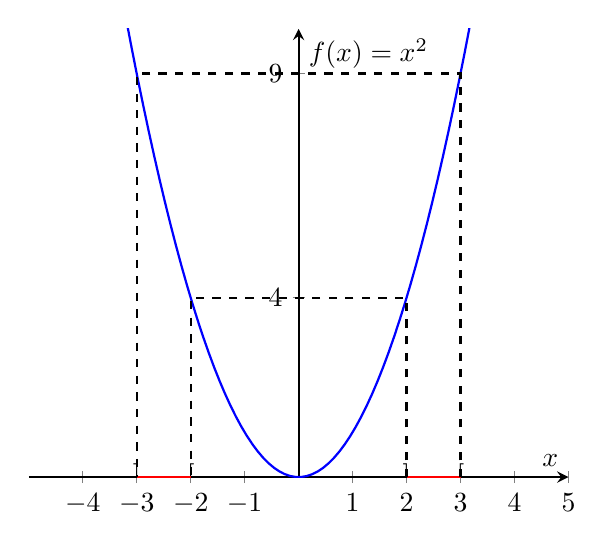
\begin{tikzpicture}
            \begin{axis}[
                axis lines = middle,
                xlabel = $x$,
                ylabel = {$f(x) = x^2$},
                xmin=-5, xmax=5,
                ymin=0, ymax=10,
                samples=100,
                domain=-5:5,
                xtick={-4,-3,-2,-1,0,1,2,3,4,5},  % Custom x-axis numbers
                ytick={0,4,9},   % Custom y-axis numbers
                thick
                ]
                \addplot[blue, thick] {x^2};
                \coordinate (a) at (2, 0);
                \node (_) at (a){$]$};
                \coordinate (b) at (-2, 0);
                \node (_) at (b){$[$};
                \coordinate (c) at (3, 0);
                \node (_) at (c){$[$};
                \coordinate (d) at (-3, 0);
                \node (_) at (d){$]$};

                \coordinate (fa) at (2, 4);
                \coordinate (fb) at (-2, 4);
                \coordinate (fc) at (3, 9);
                \coordinate (fd) at (-3, 9);
                \draw[color=red] (a) -- (c);
                \draw[color=red] (b) -- (d);

                \draw[dashed] (a) -- (fa) -- (fb) -- (b);
                \draw[dashed] (c) -- (fc) -- (fd) -- (d);
            \end{axis}
        \end{tikzpicture} 
        \caption{Exemple en $f(x) = x^2$}
    \end{figure}
\end{eg}

\chapter{Fonctions de plusieurs variables}
\section{Introduction}
\underline{Cadre:} $\R^n, \R^p$ $D \subset \R^n$
\[
F:D \to \R^p
\] 
sur $\R^n$, $\R^p$ distances usuelles, sur $D$ la distance héritée de  $\R^n$.
% \begin{figure}[ht]
%     \centering
%     \incfig{d-distance-exemple}
%     \caption{d-distance-exemple}
%     \label{fig:d-distance-exemple}
% \end{figure}

avec des coordonnées cartésiennes
\[
F(x_1, \ldots, x_n) = (F_1(x_1, \ldots, x_n), F_2(x_1, \ldots, x_n), \ldots, F_p(x_1, \ldots, x_n))
\] 
où $F_i: D \to \R$

\[
F: D \to \R^p \text{ continue}
\] 

on connaît:
\begin{lemma}
   \[
   F: D \to  \R^p \text{ continue ssi:}
   \]  
   chaque $F_i: D \to \R$ est continue
\end{lemma}
\begin{preuve}
    $Y_n = (Y_{1,n}, \ldots, Y_{p, n})$  suite des $\R^p$. $Y_n \to Y$ ssi $Y_{i,n} \to Y_i$ ($1 \le i \le p$)
\end{preuve}
\begin{prop}
   Soit $f, g: D \to \R$ continue. 
   \begin{itemize}
       \item $f + g, f \times g$ sont continues sur $D$
       \item si  $g(X) \neq 0, \: \forall X \in D, \frac{f}{g}$ continue sur $D$
       \item si  $f(D) \subset I$ intervalle et $\phi: I \to \R$ continue, alors $\phi \circ f: D \to \R$ est continue.
       \item 
           \[
               P: X \to \sum_{\alpha_1 + \ldots + \alpha_n \le d}^{} a_{\alpha_1, \ldots, \alpha_n}x^{\alpha_1} \ldots x^{\alpha_n}
           \] 
           $a_{\alpha_1, \ldots, \alpha_n} \in \R, d = \text{ degré de } P$. 
           \par
           $P: \R^n \to \R$ continue.
   \end{itemize}
\end{prop}
\section{Comment montrer qu'un ensemble est ouvert ou fermé}
D'apres la proposition ~\ref{prop:continuité-de-fonctions}, si $f: D \to Q$ est continue et $K \subset Q$ ouvert et $K_f \subset Q fermé$, donc:
\begin{itemize}
    \item $f^{-1}(K)$ est aussi ouvert
    \item $f^{-1}(K_f)$ est aussi fermé
\end{itemize}
Cela nous permet de simplifier les preuves qu'un ensemble est fermer ou ouvert. Voici quelques exemples:
\begin{eg}
   \[
       D = \{(x_1, x_2, x_3): x_1^2 + 2x_2x_3^2 < 2, \sin(x_1x_2) > 0\}
   \]  
   \[
   D = D_1 \cap D_2
   \] 
   \begin{align*}
       &D_1 = f_1^{-1}(]-\infty, 2[) &f_1(x) = x_1^2 + 2x_2x_3^2\\
       &D_2 = f_2^{-1}(]0, +\infty[) &f_2(x) = \sin(x_1x_2)
   \end{align*}
   $D_1, D_2$ sont ouverts, donc $D$ ouvert.
\end{eg}
\begin{eg}
   \[
       D = \{(x_1, x_2): \frac{e^{x_1 - 2x_2^2}}{x_1^2 + 3x_2^4} \ge 1 \}
   \]  
   \begin{align*}
       &D = f^{-1}([1, +\infty[) &f(x) = \frac{e^{x_1 - 2x_2^2}}{x_1^2 + 3x_2^4}
   \end{align*}
   $[1, +\infty[$ est fermé dans $\R$, alors D est aussi fermé car $f$ continue sur  $[1, +\infty[$
\end{eg}

\section{Lien avec la compacité}
\begin{theorem}
    Soit $F: \R^n \to \R^p$ continue et $K \subset \R^n$ compact. Alors, $F(K)$ est compact dans  $\R^p$
\end{theorem}
\begin{remark}
    On peut remplacer $\R^n, \R^p$ par $E, F$ \underline{espaces métriques}.
\end{remark}
\begin{remark}
   $U$ ouvert,  $f$ continue $\not\implies f(U)$ ouvert:
\end{remark}
\begin{eg}
   \[
       f(]0, 1[) = [-1, 1]
   \]  
   \[
   f(x) = \sin(2\pi x)
   \] 
\begin{figure}[H]
    \centering
    \incfig{exemple-ouvert-nimplique-pas-image-ouvert}
    \caption{Exemple qu'une image de l'ouvert n'est pas ouvert}
    \label{fig:exemple-ouvert-nimplique-pas-image-ouvert}
\end{figure}
\end{eg}
\begin{eg}
   \begin{align*}
       f: \R &\longrightarrow \R \\
       x &\longmapsto f(x) = \arctan x
   .\end{align*} 
   \[
       f(\underbrace{]-\frac{\pi}{2}, \frac{\pi}{2}[}_{\text{pas compact}}) = \underbrace{\R}_{\text{pas compact}}
   \] 
\end{eg}
\begin{preuve}
    Soit $(v_n)_{n \in \N}$ une suite dans $F(K)$. On a:  $v_n = F(u_n)$ où  $u_n \in K$.  $(u_n)_{n \in \N}$ suite dans $K$,  $K$ compact, donc:  $\exists$ sous suite $(u_{\phi(n)})_{n \in \N}$ avec 
    \[
        u_{\phi_n} \xrightarrow[n \to +\infty]{} u \in K
    \] 
    $F$ continue: donc  $F(u_{\phi(n)}) = v_{\phi(n)} \to F(u) \in K$. $(v_n)$ a une sous suite  $(v_{\phi(n)})$ qui converge vers $F(u) \in F(K)$, donc $F(K)$ compact!
\end{preuve}
\begin{theorem}
    Soit $F: \R^n \to \R$ continue et $K \subset \R^n$ compact. Alors $f$ est bornée sur  $K$ et atteint ses bornes. I.e, $Q := f(K)$ est bornée et atteint les bornes.
\end{theorem}
\begin{preuve}
    \underline{Weierstrass:} $f: \R \to \R$ $K = [a, b]$. \par
    Je prends  $(E, d)$ à la place de  $\R^n$. $f$ bornée sur  $K$:  $\exists c_1, c_2$ telles que 
    \[
    c_1 \le f(x) \le c_2, \forall x \in K \iff f(K) \subset [c_1, c_2] 
\] 
    C'est clair car $f(K)$ est compact dans  $\R$, donc  bornée.
    \par
    \begin{align*}
        &m = \underset{x \in K}{inf} f(x) = inf \: f(K) &M = \underset{x \in K}{sup} f(x) = sup \: f(K)
    \end{align*}
    À montrer: $\exists x \in K$ tel que $f(x) = m$ et  $\exists x' \in K$ tel que $f(x') = M$
    \par
     $m = inf \: f(K)$, ça veut dire que 
      \begin{enumerate}
          \item $f(K) \subset [m, +\infty[$ ($m$ minorant de  $f(K)$)
          \item $\forall \epsilon > 0, \exists y \in f(K)$ tel que $y \le m + \epsilon$
     \end{enumerate}
     $\epsilon = \frac{1}{n}$ donne une suite $y_n \in f(K)$ telle que $y_n \to m$
     \begin{align*}
         &y_n = f(x_n) &x_n \in K
     \end{align*}
     $K$ compact:   $\exists$ sous suite     $x_{\phi(n)}$ telle que 
      \[
      x_{\phi(n)} \xrightarrow[n \to \infty]{} x \in K
      \] 
     $f: E \to \R$ continue, donc 
     \[
         f(x_{\phi(n)}) = y_{\phi(n)} \to f(x) 
     \] 
     Mais, $y_n \to m$, donc $y_{\phi(n)} \to m$ et $y_{\phi(n)} \to f(x)$, donc $m = f(x)$,  $m$ est atteint.
     \par
     Pour montrer que $M$ est atteint la preuve est identique.
\end{preuve}

\section{Continuité partielle (inutile)}
\begin{align*}
    D \subset \R^n  \quad f: D \to \R \text{ continue} \quad D \text{ ouvert}
\end{align*}
% \begin{figure}[H]
%     \centering
%     \incfig{continuite-partielle}
%     \caption{continuite-partielle}
%     \label{fig:continuite-partielle}
% \end{figure}
Soit  $A = (a_1, \ldots, a_n) \in D$, il existe des intervalles ouverts $I_1, \ldots, I_n$ avec $a_i \in I_i$ tels que $I_1 \times \ldots \times I_n \subset D$ 
\par
Je peux poser 
\[
f_i(t) = f(a_1, \ldots, a_{i-1}, t, a_{i+1}, \ldots, a_n) \qquad t \in I_i
\] 
\begin{eg}
   \[
   n = 2 \quad f_1(t) = f(t, a_2) \quad f_2(t) = f(a_1, t)
   \]  
\begin{figure}[H]
    \centering
    \incfig{n-est-2-continuite-partielle}
    \caption{$f$ est continue en  $A = (a_1, a_2)$}
    \label{fig:n-est-2-continuite-partielle}
\end{figure}
\end{eg}

\begin{definition}
    $f$ est partiellement continue en  $A = (a_1, \ldots, a_n)$ si les $f_i(t)$ sont continues en  $a_i$ $(1 \le i \le n)$
\end{definition}
\begin{itemize}
    \item 
\underline{continuité:} $f(x_1, x_2) \xrightarrow[(x_1, x_2) \to (a_1, a_2)]{}  f(a_1, a_1)$  
    \item 
\underline{partielle:} $f(x_1, a_2) \xrightarrow[x_1 \to a_1]{}   f(a_1, a_2)$ et $f(a_1, x_2) \xrightarrow[x_2 \to a_2]{}  f(a_1, a_2)$
    \item 
\underline{Bonne notion:} continuité implique la continuité partielle (réciproque fausse)
\end{itemize}
\begin{eg}
\[
f(x_1, x_2) = \begin{cases}
    \frac{x_1x_2}{x_1^2 + x_2^2} \text{ si } (x_1, x_2) \neq (0, 0)\\
    0 \text{ si } (x_1, x_2)=(0, 0)
\end{cases}
\]     
\begin{itemize}
    \item continue sur $\R^2 \setminus \{(0, 0)\}$
    \item partiellement continue en $(0, 0)$
         \[
        f(x_1, 0) = \begin{cases}
            0 \text{ si } x_1 = 0\\
            0 \text{ si } x_1 \neq 0
        \end{cases}
        \] 
        \[
        f(0, x_2) = 0 \, \forall x_2
        \] 
    \item pas continue en $(0, 0)$:
         \[
        x_1 = r \cos(\theta) \quad x_2 = r \sin(\theta)
        \] 
        \[
        f(r\cos(\theta), r\sin(\theta)) = \begin{cases}
            0 \text{ si } r = 0\\
            \frac{r^2\cos(\theta)\sin(\theta)}{r^2} = \cos(\theta)\sin(\theta) \text{ si } r \neq 0
        \end{cases}
        \] 
        \[
        \lim_{r \to 0} f(r\cos(\theta), r\sin(\theta)) = \cos(\theta)\sin(\theta) \neq 0 \text{ si } \theta \neq 0, \pi, \frac{\pi}{2}, \ldots
        \] 
\end{itemize}
\end{eg}



\chapter{Dérivation des fonctions de plusieurs variables}
\section{Introduction}
$n = 1$: comment définir  $f'(x_0)$?
\begin{enumerate}
    \item $f'(x_0) = \lim_{x \to x_0} \frac{f(x) - f(x_0)}{x - x_0}$
    \item DL: $f(x) = f(x_0) + a_1(x - x_0) + (x - x_0)\epsilon(x)$ où $a_1 = f'(x_0)$
\end{enumerate}

\[
f: D \to R \quad D \text{ ouvert } \quad X_0 \in D \quad D \subset \R^n
\] 

\begin{definition}
    $f$ est dérivable en  $X_0$ dans la direction $\vec{u}$ $(\neq \vec{0})$ si la fonction
    \begin{align*}
        g: \R &\longrightarrow \R \\
        t &\longmapsto g(t) = f(X_0 + t\vec{u})
    .\end{align*}
    est dérivable en $t = 0$
\end{definition}
Autrement dire, la dérivée directionnelle (dans la direction de vecteur $\vec{u}$) est donnée par:
\begin{equation}\label{eq:derivee-directionnelle}
    D_{u}f(X_0) = \lim_{t \to 0} \frac{f(X_0 + t\vec{u}) - f(X_0)}{t}
\end{equation}
Dans le cas $\R$ on a eu la définition de la dérivée:
\[
f'(x_0) = \lim_{t \to 0} \frac{f(x_0 + t) - f(x_0)}{t} 
\] 
La diréction était toujours la même (l'axe $x$), on peut voir ça comme prendre un vecteur $u = (1)$ et utiliser comme la direction seulement l'axe $x$ et on obtient  l'eq. (~\ref{eq:derivee-directionnelle})
\begin{figure}[H]
    \centering
    \incfig{continuite-multidimensionelle}
    \caption{Dérivée directionnelle}
    \label{fig:continuite-multidimensionelle}
\end{figure}
$\vec{e_1}, \ldots, \vec{e_n}$ base canonique de $\R^n$, $f$ admet des dérivées partielles en  $X_0$ si $f$ dérivable en  $X_0$ dans les directions $\vec{e_1}, \ldots, \vec{e_n}$.
\[
    \frac{d}{dt} f(X_0 + t \vec{e_i}) \mid_{t = 0}
\] 
noté
\[
\frac{\partial f}{\partial x_i}(X_0)
\] 
Par contre, une fonction peut être dérivable dans \underline{toutes les diréctions} en un point mais \underline{ne pas être} continue en ce point, voici 

\begin{eg}
   \[
   f(x_1, x_2) = \begin{cases}
       1  \text{ si } x_2 = x_1^2 \text{ et } (x_1, x_2) \neq (0, 0)\\
       0 \text{ sinon}
   \end{cases}
   \]  
\begin{figure}[H]
    \centering
    \incfig{exemple-dervie-partielle}
    \caption{Exemple dérivable mais pas continue}
    \label{fig:exemple-dervie-partielle}
\end{figure}
\[
    f((0, 0) + t \vec{u}) = f(t \vec{u}) = 0
\] 
si $t\neq 0$ et $t$ petit, on a $f$ dérivable dans toutes les directions.
\par
Mais, $f$ n'est pas continue en  $(0, 0)$:
 \[
X_n = (\frac{1}{n}, \frac{1}{n^2}) \quad X_n \to (0, 0)
\] 
\[
\forall n, f(X_n) = 1 \quad f(X_n) \not\xrightarrow[n \to \infty]{} f(0, 0)
\] 
\end{eg}

\begin{definition}\label{def:fonction-differentiable}
    Soient $D \subset \R^n$ ouvert et $X_0 \in D$, la fonction
    $f: D \to \R$
    est \textbf{différentiable} en $X_0$ s'il existe un vecteur $\vec{u} \in \R^n$ tel que 
    \[
        f(X_0 + \vec{X}) = f(X_0) + \vec{u} \cdot \vec{X} + \|\vec{X}\|\epsilon(\vec{X})
    \] 
    où $\lim_{\vec{X} \to \vec{0}} \epsilon(\vec{X}) = 0$
\end{definition}
\begin{intuition}
   Je propose de réflechir sur ce que cette définition signifie. 
   Rappelons ce que signifie intuitivement la dérivée au cas $\R^n = \R$ ($n = 1$). 
   Intuitivement, si on zoom la fonction qu'on dérive elle se comporte et a l'air d'être une ligne. 
   Dans le cas $R^n = \R^2$, si on zoom la fonction elle a l'air d'être un plan. 
   En effet, c'est ça l'idée de la dérivée, que si on fait un petit petit pas d'un fourmit, le deplacement et aussi petit et uniforme. 
   En augmentant $n$, la dérivée donne des scalaire pour contruire un sous-éspace de dimension $n-1$ de l'espace $\R^n$. 
\end{intuition}
\begin{note}
   Pour montrer qu'une fonction est différentiable il suffit de montrer que ces dérivées partielles sont continues. 
\end{note}

\section{DL à l'ordre 1}
Cette représentation de la dérivée comme un sous-éspace lorsqu'on zoom est représenté par le DL à l'ordre $1$.
De la définition ~\ref{def:fonction-differentiable}, ce vecteur $\vec{u}$ se note $\vec{\nabla}f(X_0)$ (gradient de $f$ en  $X_0$)

\begin{prop}
   $f$ différentiable en  $X_0$ $\implies$ $f$ dérivable dans toutes les directions en  $X_0$, et alors: 
   \[
       \vec{\nabla}f(X_0) = \begin{pmatrix} \frac{\partial f}{\partial x_1}f(X_0)\\ \ldots \\  \frac{\partial f}{\partial x_n}f(X_0)\end{pmatrix} 
   \] 
   dans la base $\vec{e_1}, \ldots, \vec{e_n}$
\end{prop}

\begin{preuve}
$f$ est continue en  $X_0$ $|\vec{u} \cdot X| \le |\vec{u}| |X|$
\begin{enumerate}
    \item continuité
        \begin{align*}
            |f(X_0 + X) - f(X_0)| &\le |\vec{u} \cdot X| + \|X\| |\epsilon(X)|\\
                                  &\le \|X\|\left( \|\vec{u}\| + |\epsilon(x)|  \right) \le c\|X\|
        \end{align*}
        donc: $f(X_0 + X) \xrightarrow[X \to \vec{0}]{} f(X_0)$
    \item .
        \begin{align*}
            g(t) = f(X_0 + t \vec{v}) &= f(X_0) + \vec{\nabla}f(X_0) \cdot t \vec{v} + \|t \vec{v}\| \cdot \epsilon(t \vec{v})\\
                                      &= f(X_0) + t\vec{\nabla}f(X_0) \cdot \vec{v} + |t|\|\vec{v}\|\epsilon_1(t)\\
                                      &= f(X_0) + t\vec{\nabla }f(X_0)\cdot \vec{v}
        \end{align*}
        donc:
        \[
            \frac{d}{dt} f(X_0 + t\vec{v})\mid_{t = 0} = \vec{\nabla}f(X_0)\cdot \vec{v}
        \] 
        (prendre $\vec{v} = \vec{e_1}, \ldots, \vec{e_n}$ pour les coordonnées de $\vec{\nabla}f(X_0)$)
\end{enumerate}
\end{preuve}
\begin{definition}
    \[
        D \subset \R^n \quad D \text{ ouvert } \quad f: D \to \R \text{ est } \mathcal{C}^1 \text{ sur } D
    \] 
    Soit $D \subset \R^n$ ouvert, alors la fonction $f: D \to \R$ est de classe $\mathcal{C}^1$ sur  $D$ si 
    $f$ est différentiable en tout  $X \in D$ et la fonction
    \begin{align*}
        : D &\longrightarrow \R^n \\
        X &\longmapsto \vec{\nabla}f(X)
    \end{align*}
    est continue.
\end{definition}
\begin{theorem}
    $f$ de classe  $\mathcal{C}^1$ sur  $D$ ssi  $f$ admet des dérivées partielles continues en tout point de  $D$. 
\end{theorem}

\begin{eg}
   \[
       f(X) = f(X_0) + \vec{\nabla}f(X_0) \cdot (X - X_0) + \|X - X_0\| \epsilon(X - X_0)
   \]  
   linéaire
   \par
   Dans $\R^3$: $f(x, y, z)$
    \[
        S = \{(x, y, z): f(x, y, z) = 0 \}
   \] 
   $S$: surface dans  $\R^3$, $X_0 \in S$ plan tangent à $S$ en  $X_0$, plan d'équation:
   \[
       f(X_0) + \vec{\nabla}f(X_0)\cdot X = 0
   \] 
\begin{figure}[H]
    \centering
    \incfig{surface-s-differentiable}
    \caption{Exemple d'une surface differentiable}
    \label{fig:surface-s-differentiable}
\end{figure}
\end{eg}
\section{Extrema et points critiques}
\begin{definition}
    Extremum (local) de $f$ est un minimum ou un maximum (local) de  $f$
    \begin{itemize}
        \item $X_0$ est un maximum local de $f$ si: $\exists \delta > 0$ tel que
            \[
            \forall X \in D, f(X) \le f(X_0) \text{ avec } d(X, X_0) \le \delta
            \] 
        \item $X_0$ est un minimum local de $f$ si: $\exists \delta > 0$ tel que
            \[
            \forall X \in D, f(X) \ge f(X_0) \text{ avec } d(X, X_0) \le \delta
            \] 
    \end{itemize}
\end{definition}

\begin{definition}
    Soit $f: D \to \R$ et $X_0 \in D$, alors si
     \[
         \vec{\nabla}f(X_0) = \vec{0}
    \] 
    donc $X_0$ est un \textbf{point critique}.
\end{definition}
\begin{intuition}
   Le lien entre les extremums et le point critique: 
   \begin{enumerate}
       \item pour que l'extremum existe, il faut qu'il existe au moins un point critique - c'est un critère nécessaire \underline{mais pas suffisant}.
       \item tout extremum local est un point critique
   \end{enumerate}
   Les points critiques falicites la recherche des extremums locaux.
\end{intuition}

\begin{theorem}
    Soit $f: D \longrightarrow \R$ différentiable, $D$ ouvert et  $X_0 \in D$ (sinon, si $D$ pas ouvert, il faut  $X_0 \in \operatorname{Int}(D)$) alors:
    \[
        X_0 \text{ extremum local } \implies X_0 \text{ point critique} 
    \] 
\end{theorem}

\begin{eg} Pas tout point critique est un extremum local
\begin{figure}[H]
    \centering
    \incfig{point-critique-nestpas-extremum-local}
    \caption{Point critique qui n'est pas un extremum local}
    \label{fig:point-critique-nestpas-extremum-local}
\end{figure}
\end{eg}

\section{Dérivées partielles d'ordre $\ge 2$}
\begin{definition}
    Soit $D$, alors  $f: D \to \R$ est $\mathcal{C}^k$ si  $f: D \to \R$ est $\mathcal{C}^1$ et  $\partial_{x_i}f: D \to \R$ sont $C^{k-1}$
\end{definition}

\begin{definition}
    Soient $\alpha = (\alpha_1, \ldots, \alpha_n)$ \quad $\alpha_i \in \N$. On pose
    \[
        \partial_{x}^{\alpha}f = \frac{\partial^{\alpha_1}}{\partial x_1^{\alpha_1}} \cdot \ldots \cdot \frac{\partial^{\alpha_n}}{\partial x_n^{\alpha_n}}
    \] 
    est la notation pour la dérivée d'ordre supérieure.
\end{definition}
\[
    \frac{\partial}{\partial x_1}\frac{\partial}{\partial x_2}\frac{\partial}{\partial x_1} f \overset{?}{=}  \frac{\partial^2}{\partial x_1^2}\frac{\partial}{\partial x_2}f
\] 

\begin{theorem}\label{thm:lemme-de-schwarz}
    Lemme de Schwarz
    \par
    Si $f \in \mathcal{C}^2(D)$ alors 
    \[
        \displaystyle \frac{\partial^2 f}{\partial x_i\partial x_j}(X) = \frac{\partial^2 f}{\partial x_j\partial x_i}(X) \qquad \forall X \in D, \forall i, j
    \] 
\end{theorem}
\begin{eg} où une fonction admet des dérivées partielles d'ordre supérieure mais $\displaystyle \frac{\partial^2 f}{\partial x_i\partial x_j}(X) \neq  \frac{\partial^2 f}{\partial x_j\partial x_i}(X)$
   \[
   f(x_1, x_2) = \begin{cases}
       x_1x_2 \frac{x_1^2 - x_2^2}{x_1^2 + x_2^2} \text{ si } (x_1, x_2) \neq (0, 0)\\
       0 \text{ si } (x_1, x_2) = 0
   \end{cases}
   \]  
   \[
   r^2 \sin(\theta)\cos(\theta)\cos(2\theta) = \frac{1}{4}r^2\sin(4\theta)
   \] 
   On calcule $\displaystyle \frac{\partial^2f}{\partial_{x_1}\partial_{x_2}}(0, 0)$?
       C'est $\displaystyle \frac{\partial}{\partial x_1}g(x_1)$ en $x_1 = 0$ pour $\displaystyle g(x_1) = \frac{\partial f}{\partial x_2}(x_1, x_2)|_{x_2 = 0}$. Calcul de $g(x_1)$:
    \begin{enumerate}
        \item si $x_1 \neq 0$ $\frac{\partial f}{\partial x_2}(x_1, x_2) = x_1 \frac{x_1 ^ 2 - x_2^2}{x_1^2 + x_2^2}$, donc si $x_1 \neq 0$ $\frac{\partial f}{\partial x_2}(x_1, 0) = x_1$ 
        \item si $x_1 = 0$ $f(0, x_2) = 0$
    \end{enumerate}
    Conclusion:
    \[
    \frac{\partial f}{\partial x_2}(x_1, 0) = x_1 \quad \forall x_1
    \] 
    donc: 
    \[
    \frac{\partial}{\partial x_1}\frac{\partial}{\partial x_2}f(0, 0) = 1
    \] 
    $\displaystyle \frac{\partial}{\partial x_2}\frac{\partial}{\partial x_1}f(0, 0) = ?$. On voit que, $f(x_2, x_1) = -f(x_1, x_2)$ donc 
    \[
    \frac{\partial}{\partial x_2}\frac{\partial}{\partial x_1}f(0, 0) = - \frac{\partial}{\partial x_1}\frac{\partial}{\partial x_2}f(0, 0) = -1
    \] 
\end{eg}

\section{Formule de Taylor à l'ordre 2}
\begin{definition}
    Soit $f \in \mathcal{C}^2(D)$. Matrice hessienne: matrice  $n \times n$
    \[
    H_f(X_0) = \begin{bmatrix} \frac{\partial^2}{\partial x_i \partial x_j}(X_0) \end{bmatrix} 1\le i,j \le n
    \] 
    Le lemme \ref{thm:lemme-de-schwarz} nous donne que $H_f(X_0)$ est symmetrique si $f \in \mathcal{C}^2(D)$
\end{definition}
Rappel: 
\[
    \vec{\nabla}f(X_0) = \begin{pmatrix} \frac{\partial f}{\partial x_1}(X_0) \\ \vdots \\ \frac{\partial f}{\partial x_n}(X_0) \end{pmatrix} 
\] 

\begin{theorem} De Taylor à l'ordre 2 \par
    Soit $f \in \mathcal{C}^2(D)$,  $X_0 \in D$. Alors  
    \begin{align*}
        f(X_0 + \vec{X}) = f(X_0) + \vec{\nabla }f(X_0) \cdot \vec{X} + \frac{1}{2}\vec{X} \cdot H_f(X_0)\vec{X}
    \end{align*}
    exemple en $\R^1$
    \[
    f(x_0 + x) = f(x_0) + f'(x_0)x + \frac{1}{2}f''(x_0)x^2 + \ldots
    \] 
\end{theorem}
\begin{intuition}
   Alors, la matrice hessienne sert à calculer la dérivée d'ordre 2. 
\end{intuition}

\section{Un rappel d'algèbre linéaire et le lien avec l'analyse}
\[
    \vec{X} \cdot A\vec{X} = \sum_{1\le i,j \le n}^{} x_ia_{i,j}x_j
\] 
Si $\vec{X} = \begin{pmatrix} x_1 \\ \vdots \\ x_n \end{pmatrix}$ $A = \begin{bmatrix} a_{i,j} \end{bmatrix}$ on a: $X \mapsto X \cdot AX$ à étudier. Si $A = A^T, A \in \mathcal{M}_n(\R)$
\begin{center}
   "$A$ admet une base orthonormée de vecteurs propres" 
\end{center}
Il existe une base $\vec{u_1}, \ldots, \vec{u_n}$ de $\R^n$ avec $\vec{u_i} \cdot \vec{u_j} = \delta_{i, j}$ ($1$ si  $i = j$ et  $0$ sinon) et des réels $\lambda_1, \ldots, \lambda_n$($\lambda_i = \lambda_j$ possible) tels que
\[
    A\vec{u_i} = \lambda_i\vec{u_i}
\] 
\[
    \vec{X} = \sum_{j=1}^{n} y_j\vec{u_j}
\] 
\[
    \vec{X} \cdot \vec{u_i} = \sum_{j=1}^{n} y_j\vec{u_j}\vec{u_i} = y_i
\] 
\begin{align*}
    \|\vec{X}\|^2 = \vec{X} \cdot \vec{X} &= \left( \sum_{j=1}^{n} y_j\vec{u_j} \right) \cdot \left( \sum_{i=1}^{n} y_i\vec{u_i} \right) \\
                                          &= \sum_{j=1}^{n} \sum_{i=1}^{n} y_jy_i\vec{u_j}\cdot \vec{u_i}\\ 
                                          &= \sum_{j=1}^{n} y_j^2
\end{align*}

\begin{align*}
    A\vec{X} = A \sum_{j=1}^{n} y_j\vec{u_j} = \sum_{j=1}^{n} y_jA\vec{u_j} = \sum_{j=1}^{n} \lambda_jy_j\vec{u_j}
\end{align*}
\[
    \vec{X} \cdot A\vec{X} = \sum_{i=1}^{n} \lambda_iy_i^2
\] 
\begin{enumerate}
    \item si $\lambda_i > 0$ ($1 \le i \le n$)
        \[
        C = \min \lambda_i > 0
        \] 
        \[
        X \cdot AX \ge C \sum_{i=1}^{n} y_i^2 = C \|X\|^2
        \] 
    \item si $\lambda_i < 0$ ($1 \le i \le n$)
        \[
        -C = \max \lambda_i < 0
        \] 
        \[
        X \cdot AX \le -C\|X\|^2
        \] 
\end{enumerate}
\begin{eg}
   $n = 2$ 
   \[
   f(y_1, y_2) = -y_1^2 + 3y_2^2
   \] 
   \[
   \lambda_1 = -1 \qquad \lambda_2 = 3
   \] 
   \[
   f(y_1, 0) < f(0, 0) < f(0, y_2)
   \] 
\end{eg}

\section{Nature des points critiques}
\begin{theorem}\label{thm:nature-des-points-critiques}
    (Nature des points critiques) \par
    Soient $f \in \mathcal{C}^2(D)$,  $X_0 \in D$, $D$ ouvert et  $\vec{\nabla }f(X_0) = \vec{0}$
    \begin{enumerate}
        \item si toutes les valeurs propres de $H_f(X_0)$ sont $> 0$ (resp $< 0$) $X_0$ est minimum (resp. maximum) local.
        \item si toutes les valeurs propres de $H_f(X_0)$ sont \underline{non nulles} mais pas de même signe, $X_0$ n'est pas un extremum local: $X_0$ est un point selle (un col).
        \item si 0 valeurs propres de $H_f(X_0)$, pas de conclusion, ($X_0$ point critique dégénéré) i.e on ne peut rien conclure
    \end{enumerate}
\end{theorem}

\begin{preuve} du théorème ~\ref{thm:nature-des-points-critiques}
   \[
       f(X_0 + X) - f(X_0) = \frac{1}{2}X\cdot H_f(X_0)X + \|X\|^2\epsilon(X)
   \]  
   .
   \begin{enumerate}
       \item si $\lambda_i > 0$  $\frac{1}{2}X \cdot H_f(X_0)X \ge C\|X\|^2$ $C > 0$
            \[
           f(X_0 + X) - f(X_0) \ge \|X\|^2(C + \epsilon(X)) \ge \frac{C}{2}\|X\|^2 \text{ si } \|X\| \text{ assez petit }
           \] 
           \[
           \implies X_0 \text{ minimum local}
           \] 
        \item si $\lambda_1 < 0$ et  $\lambda_2 > 0$
             \[
                 H_f(X_0)\vec{u_i} = \lambda_i\vec{u_i}
            \] 
            \[
                f(X_0 + t\vec{u_i}) = f(X_0) + \frac{1}{2} \lambda_it^2 + t^2\epsilon(t)
            \] 
            \[
                \epsilon(t\vec{u_i}) = \epsilon(t)
            \] 
            \[
                f(X_0 + t\vec{u_i}) - f(X_0) = t^2 (\frac{1}{2}\lambda_i + \epsilon(t))
            \] 
            si $i = 1$  $< 0$  $|t|$ petit,  $i = 2$  $> 0$  $|t|$ petit, alors  $X_0$ n'est pas un extremum local
   \end{enumerate}
\end{preuve}

\begin{eg}
   \[
   f(x, y) = \frac{1}{2}(x^2 - y^2)
   \]  
   \[
       H_f(0, 0) = \begin{pmatrix} 1 & 0\\ 0 & -1 \end{pmatrix} 
   \] 
   \[
       I_f = \{(x, y, z): z = \frac{1}{2}(x^2 - y^2)\}
   \] 
\begin{figure}[H]
    \centering
    \incfig{exemple-point-selle}
    \caption{Exemple de point selle.}
    \label{fig:exemple-point-selle}
\end{figure}
Les lignes rouges représentent les dérivées partielles et on voit bien que les uns sont croissants et les autres décroissants, donc ce point n'est ni le minimum ni le maximum
\end{eg}

\begin{eg}
$n = 2$
 \[
A = \begin{pmatrix} 
    a_{1,1} & a_{1, 2}\\
    a_{2, 1} & a_{2, 2}
\end{pmatrix} 
\] 
$(a_{1,2} = a_{2, 1})$
\par
Valeurs propres: racines du pol. Caractéristique:  
\[
    P(\lambda) = \det(A - \lambda I) = \begin{vmatrix} a_{1,1} - \lambda & a_{1, 2} \\ a_{2, 1} & a_{2,2} - \lambda \end{vmatrix} = (\lambda - a_{1,1})(\lambda - a_{2,2}) -  a_{1,2}a_{2,1}
\] 
\[
    \lambda^2 - (a_{1,1} + a_{2,2})\lambda + a_{1,1}a_{2,2} - a_{2,1}a_{1,2}
\] 
\[
    a_{1,1} + a_{2,2} = Tr(A)
\] 
\[
    a_{1,1}a_{2,2} - a_{2,1}a_{1,2} = \det(A)
\] 
\[
    x^2 - Sx + P = x^2 - (\lambda_1 + \lambda_2)x + \lambda_1\lambda_2
\] 
\begin{align*}
    &\det(A) = \text{ produit des valeurs propres}\\
    &Tr(A) = \text{ somme des valeurs propres}
\end{align*}
\[
A = H_f(X_0)
\] 
\begin{enumerate}
    \item si $\det(A) < 0$,  $X_0$ point col
    \item si $\det(A) > 0$
         \begin{enumerate}
            \item $Tr(A) > 0$, $X_0$ minimum
            \item  $Tr(A) < 0$, $X_0$ maximum
        \end{enumerate}
    \item $\det(A) = 0$,  $X_0$ point critique dégénéré
\end{enumerate}
\end{eg}

\section{La règle de dérivation en chaîne}

\begin{definition}
Soit $f: \R^n \to \R$ une fonction continue est différentiable et des fonction $g_1: \R \to \R$, $\ldots$, $g_n: \R \to \R$ des fonctions dérivables et continues et  
\begin{align*}
    h: \R &\longrightarrow \R \\
    t &\longmapsto h(t) = f(g_1(t), g_2(t), \ldots, g_n(t))
\end{align*}
alors 
\[
h'(t) = \frac{\partial g_1}{\partial h}g_1'(t) + \frac{\partial g_2}{\partial h}g_2'(t) + \ldots + \frac{\partial g_n}{\partial h}g_n'(t)
\] 
\end{definition}

\begin{definition}
Soit $f: \R^n \to \R$ une fonction continue est différentiable et des fonction $g_1: \R^p \to \R$, $\ldots$, $g_n: \R^p \to \R$ des fonctions dérivables 
i.e 
\begin{align*}
    \forall i \in \{ 1, \ldots, n\}, \quad
    g_i : \R^p &\longrightarrow \R \\
    (t_1, \ldots, t_n)&\longmapsto g_i(t_1, \ldots, t_n) 
\end{align*}
et  
\begin{align*}
    h: \R^n &\longrightarrow \R \\
    (x_1, \ldots, x_n) &\longmapsto h(g_1(t_1, \ldots, t_p), \ldots, g_n(t_1, \ldots, t_p)) 
.\end{align*}
donc 
\[
\frac{\partial h}{\partial t_i} = \frac{\partial h}{\partial x_1}\frac{\partial g_1}{\partial t_i} + \ldots + \frac{\partial h}{\partial x_n}\frac{\partial g_n}{\partial t_i}
\] 
\end{definition}
% \chapter{Espaces vectoriels normés}
Soient:
\begin{itemize}
    \item espace vectoriel $E$,  $F$, etc
    \item vecteurs:  $x, y, e$, etc.
    \item vecteur nul: noté  $0_E$ ou simplement  $0$
    \item scalaires:  $\lambda, \mu \in \mathbb{K}$
    \item  $\mathbb{K} = \R \text{ ou } \mathbb{C}$
    \item $A \in \mathcal{L}(E, F)$ action sur $x$, notée  $Ax$ (plutôt que $A(x)$)
    \item dimension: $E$ de dimension finie si  $E$ admet une base avec un nombre fini d'éléments, sinon  $E$ est dit de dimension infinie  $\iff$ $\forall N \in \N$, il existe une famille libre de $N$ vecteurs. La dimension dépend de  $\mathbb{K}$!
         \begin{itemize}
             \item sur $\mathbb{C}$  $\dim \mathbb{C} = 1$ base formée du vecteur  $1 \in \mathbb{C}$
             \item sur  $\R$ $\dim \mathbb{C} = 2$ base formée de $1, i$
        \end{itemize}
        \begin{align*}
            &z = z \cdot 1 \quad z \in \mathbb{C}\\
            &z = x \cdot 1 + y \cdot i \quad x, y \in \R
        \end{align*}
        \[
            \mathbb{C} \sim \R^2 \text{ comme } \R \text{ espace vectoriel}
        \] 
\end{itemize}

\chapter{Espaces vectoriels normés}
\section{Introduction}
\begin{definition}
    Soit $E$ un  $\mathbb{K}$-espace vectoriel et $\lambda \in \R$, la \textbf{norme} sur  $E$ est une application $N: E \to \R_{+}$ avec:
    \begin{enumerate}
        \item $N(\lambda u) = |\lambda|N(u) \quad u \in E$
        \item $N(u + v) \le N(u) + N(v)$
        \item $N(u) = 0 \iff u = 0_{E}$
    \end{enumerate}
    \textbf{semi-norme}: $1$ et  $2$ seulement.
\end{definition}

On peut interpreter $2$ comme:
 \[
\left| N(u) - N(v) \right| \le N(u - v)
\] 

\begin{prop}
    \textbf{Norme induite}: Si $F \subset E$ un sous-espace vectoriel, je restreins $N$ à  $F$, alors  $(F, N)$ est un espace vectoriel normé.
\end{prop}

\begin{eg}
    $E = \mathbb{K}^n$ avec  $x = (x_1, \ldots, x_n) \in E$ 
    \begin{itemize}
        \item $\|x\|_1 = \sum_{i=1}^{n} |x_i|$
        \item $\|x\|_2 = \left(\sum_{i=1}^{n} |x_i|^2\right)^{\frac{1}{2}}$
        \item $\|x\|_{\infty} = \max_{1 \le i \le n} |x_i|$
        \item $\|x\|_p = \left( \sum_{i=1}^{n} |x_i|^p \right)^{\frac{1}{p}}$ avec $1 \le p < \infty$
    \end{itemize}
\end{eg}

\begin{prop}
    L'inégalité triangulaire pour $p > 2$ s'appelle \textbf{l'inégalité de Minkowski}:
    \[
        \left( \sum_{i=1}^{n} |x_i + y_i|^p \right)^{\frac{1}{p}} \le  \left( \sum_{i=1}^{n} |x_i |^p \right)^{\frac{1}{p}} + \left( \sum_{i=1}^{n} |y_i|^p \right)^{\frac{1}{p}}
    \] 
\end{prop}

\begin{definition}
    Soit $U$ un ensemble et $E = \{f: U \to \mathbb{K} \text{ bornée} \}$ 
    \[
        \|f\|_{\infty} = \sup_{x \in U} |f(x)| \text{ norme sur E}
    \] 
\end{definition}
\begin{definition}
    $R([a, b], \mathbb{K})$ = $\{$ les  $f: [a, b] \to \mathbb{K}$ intégrables au sens de Riemann\footnote{La fonction est Riemann intégrable (pas forcément continue) si on peut calculer l'air en utilisant l'intégration par les sommes de Riemann. Alors, si $f$ discontinue, elle est Riemann intégrable si la discontinuité est négligable.} $\}$
\end{definition}

\begin{eg}
    \[
        \|f\|_{p} = \left( \int_{{a}}^{{b}} {|f(x)|^{p}} \: d{x} {} \right)^{\frac{1}{p}} \text{ avec } 1 \le p < \infty
    \] 
    $\| . \|_{p}$ est une semi-norme sur $R([a, b], \mathbb{K})$ (inégalité de Minkowski). $\|f\|_{p} = 0$ n'entraine pas que $f = 0$ (e.g: $[a, b] = [-1, 1]$,  $f(x) = x$, $p = 3$). 
    \[
        \|u + v\|_{p} \le \|u\|_p + \|v\|_p
    \] 
    Sur $E = \mathcal{C}([a, b], \mathbb{K})$,  $\| . \|_{p}$ est une norme:
    si $f: [a, b] \to \mathbb{K}$ continue et $\int_{{a}}^{{b}} {|f(x)|^p} \: d{x} = 0$ alors $f(x) = 0 \forall x \in [a, b]$
\end{eg}

\begin{eg}
    $E = \mathbb{K}^{\N}$ un ensemble des suites $u$ à valeurs dans  $\mathbb{K}$ 
    \[
    u = (u_1, u_2, \ldots, u_n, \ldots )
    \] 
    pour $1 \le p < \infty$
    \[
        l^{p}(\N, \mathbb{K}) = \{(u_n): \sum_{n \in \N}^{} |u_n|^{p} \text{ est convergente } \}
    \] 
    \[
        \|u\|_p = \left( \sum_{n=0}^{\infty} |u_n|^{p} \right)^{\frac{1}{p}}
    \] 
    est une norme sur $l^{p}(\N, \mathbb{K})$
    \[
        p = \infty \quad l^{\infty}(\N, \mathbb{K}) = \{u \text{ bornée } \}
    \] 
    \[
        \|u\|_{\infty} = \sup_{n \in \N} |u_n|
    \] 
\end{eg}
\section{Topologie des espaces vectoriels normés}
\begin{prop}
    Soit $(E, \| . \|)$ un espace vectoriel normé avec 
     \[
    d(u, v) = \|u - v\|
    \] 
    une distance sur $E$ (induite par $\| . \|$), alors  $(E, d)$ est un espace métrique.
\end{prop}
\begin{definition}
    Un espace vectoriel normé complet s'appelle \textbf{un espace de Banach}.
\end{definition}
Cas de dimension finie:
\begin{enumerate}
    \item Tout espace vectoriel normé de dimension finie est complet (rappel: proposition \ref{prop:rd-est-complet}) (voir plus bas)
    \item Si $E$ de dim finie:
         \[
        K \text{ compact} \iff K \text{ fermé et borné }
        \] 
\end{enumerate}
\begin{lemma}
   \[
       \left( \mathcal{C}([0, 1], \R), \|.\|_1 \right) 
   \]  
   n'est pas complet.
\end{lemma}
\begin{preuve}
    On construit une suite de fonctions continues $(f_n)_{n \in \mathbb{N}}$ sur $[0,1]$ qui converge en norme $\| \cdot \|_1$ vers une fonction $f$ discontinue. Cela montrera que la limite de cette suite dans la norme $\| \cdot \|_1$ n’appartient pas à $\mathcal{C}([0,1], \mathbb{R})$, donc que cet espace n’est pas complet.
    
\begin{figure}[H]
    \centering
    \incfig{lemma-n-est-pas-complet}
    \caption{Lemma avec un espace pas complet}
    \label{fig:lemma-n-est-pas-complet}
\end{figure}

\medskip

\textbf{Définition de la suite $(f_n)$ :} pour chaque $n \in \mathbb{N}$, on définit $f_n : [0,1] \to \mathbb{R}$ par
\[
f_n(x) = 
\begin{cases}
0 & \text{si } x \le \frac{1}{2} - \frac{1}{2n}, \\[4pt]
2n\left(x - \frac{1}{2} + \frac{1}{2n}\right) & \text{si } \frac{1}{2} - \frac{1}{2n} < x < \frac{1}{2} + \frac{1}{2n}, \\[4pt]
1 & \text{si } x \ge \frac{1}{2} + \frac{1}{2n}.
\end{cases}
\]
Chaque $f_n$ est continue sur $[0,1]$ car elle est affine par morceaux avec raccords continus.

\medskip

\textbf{Définition de la fonction limite :} posons
\[
f(x) = 
\begin{cases}
0 & \text{si } x < \frac{1}{2}, \\
1 & \text{si } x > \frac{1}{2}, \\
\text{valeur quelconque} & \text{si } x = \frac{1}{2}.
\end{cases}
\]
Alors $f$ est \textbf{discontinue} en $x = \frac{1}{2}$, donc $f \notin \mathcal{C}([0,1], \mathbb{R})$.

\medskip

\textbf{Convergence de $(f_n)$ vers $f$ dans $\| \cdot \|_1$ :}

On a
\[
\|f_n - f\|_1 = \int_0^1 |f_n(x) - f(x)|\, dx.
\]
Mais $f_n(x) = f(x)$ sauf sur l’intervalle $\left[\frac{1}{2} - \frac{1}{2n}, \frac{1}{2} + \frac{1}{2n}\right]$ de longueur $\frac{1}{n}$, et sur cet intervalle, $|f_n(x) - f(x)| \le 1$, donc :
\[
\|f_n - f\|_1 \le \int_{\frac{1}{2} - \frac{1}{2n}}^{\frac{1}{2} + \frac{1}{2n}} 1\, dx = \frac{1}{n} \xrightarrow[n \to \infty]{} 0.
\]

Ainsi, $f_n \to f$ dans la norme $\| \cdot \|_1$.

\medskip

\textbf{Conséquence :} la suite $(f_n)$ est de Cauchy dans $\left( \mathcal{C}([0,1], \mathbb{R}), \| \cdot \|_1 \right)$, car :
\[
\|f_n - f_p\|_1 \le \|f_n - f\|_1 + \|f - f_p\|_1 \le \frac{1}{n} + \frac{1}{p} \xrightarrow[n,p \to \infty]{} 0.
\]

Cependant, la limite $f$ n’est pas continue, donc $f \notin \mathcal{C}([0,1], \mathbb{R})$.

\medskip

\textbf{Conclusion :} Il existe une suite de Cauchy dans $\left( \mathcal{C}([0,1], \mathbb{R}), \| \cdot \|_1 \right)$ qui ne converge pas dans cet espace. Par conséquent, cet espace n’est pas complet.

\end{preuve}
\begin{lemma}
    Dans $E = l^{1}(\N, \R)$ muni de
    \[
    \|u\|_1 = \sum_{n=0}^{\infty} |u_n|
    \] 
    $B_f(0, 1)$ n'est pas compact.
\end{lemma}
\begin{preuve}
    On construit une suite d'éléments de $B_f(0, 1)$ \underline{sans sous-suite convergente}.
    \[
    u \in E \quad u: \N \to \R
    \] 
    Je note $u(p)$ au lieu de  $u_p$ suite dans  $E$ noté  $(u_n)$,  $u_n \in E$. $u_n(p)$ p-ième terme de  $u_n$. Je pose  
    \[
    u_n(p) = \delta_{n, p} = \begin{cases}
        1 \text{ si } n = p\\
        0 \text{ sinon}
    \end{cases}
    \] 
    \[
    \|u_n\|_1 = \sum_{p=0}^{\infty} |u_n(p)| = |u_n(n)| = 1
    \] 
    Donc $u_n \in B_f(0, 1) \forall n$.
    \par
    Si $v \in l^1(\N, \R)$
    \[
    |v(p)| \le \sum_{p=0}^{\infty} |v(p)| = \|v\|_1
    \] 
    si $\|v_n - v\|_1 \xrightarrow[n \to \infty]{} 0$ alors $\forall p, v_n(p) \to v(p)$. Supposons que $(v_n) = (u_{\phi(n)})$ est une sous-suite de $(u_n)$ qui converge vers  $v$ pour  $\| . \|$. Je fixe $p \in \N$, $v_n(p) = u_{\phi(n)}(p) \xrightarrow[n \to \infty]{} v(p)$, mais $v_n(p) \xrightarrow[n \to \infty]{} 0$, donc $v(p) = 0 \forall p$. $v$: suite nulle, aussi 
     \[
    \|v_n\|_1 = 1 \forall n \text{ et } \|v_n\|_1 \xrightarrow[n \to \infty]{} \|v\|_1
    \] 
    contradiction
\end{preuve}
\section{Normes équivalentes}
\begin{definition}
    Deux normes $N_1$ et  $N_2$ sur  $E$ sont équivalentes ($N_1 \sim N_2$) si $\exists c_1, c_2 > 0$ telles que 
    \begin{itemize}
        \item $N_1(u) \le c_1N_2(u) \quad \forall u \in E$
        \item $N_2(u) \le c_2N_1(u) \quad \forall u \in E$
    \end{itemize}
    $\exists c > 0$ telle que
    \[
    cN_1(u) \le N_2(u) \le cN_1(u)
    \] 
\end{definition}
\begin{remark}
   Si  $N_1 \sim N_2$ et $N_2 \sim N_3$, alors $N_1 \sim N_3$ 
\end{remark}
\begin{definition}
    Les normes $N_1$ et $N_2$ sont \textbf{topologiquement équivalentes} si elles définissent les mêmes ensembles ouverts.
\end{definition}
\begin{theorem}
    Soientt $N_1, N_2$ deux normes, alors:
    \[
    N_1, N_2 \text{ topologiquement équivalentes } \iff N_1, N_2 \text{ équivalentes }
    \] 
\end{theorem}
\begin{eg}
    \begin{enumerate}
        \item $E = \mathcal{C}([0, 1], \R)$
        \item $\|f\|_{\infty} = \sup_{x \in [0, 1]}|f(x)|$
        \item $\|f\|_1 = \int_{{0}}^{{1}} {|f(x)|} \: d{x}$
    \end{enumerate}
    On remarque que $\|f\|_1 \le \|f\|_{\infty}$. Est-ce que $\exists c > 0$ telle que 
    \[
    \|f\|_{\infty} \le c\|f_1\| \forall f \in E
    \] 
    ?
    Pour le voir, construire une suite $(f_n)$ dans  $E$ telle que  $\|f_n\|_1 \to 0$ mais $\|f_n\|_{\infty} \not\to 0$
\end{eg}
\begin{theorem}
    Soit $E$ un espace de dimension finie. Alors toutes normes sur  $E$ sont équivalentes.
\end{theorem}
\begin{preuve}

   Puisque \( E \) est de dimension finie, il existe une base de \( E \) et donc un isomorphisme linéaire entre \( E \) et \(\mathbb{R}^n\) (ou \(\mathbb{C}^n\)). En conséquence, on peut se ramener à l'étude de normes sur \(\mathbb{R}^n\).


   Considérons la norme \(\|\cdot\|_1\) sur \( E \) et définissons la sphère unité associée :
   \[
   S = \{ x \in E : \|x\|_1 = 1 \}.
   \]
   Dans un espace de dimension finie, la sphère unité \( S \) est compacte (cela repose sur le fait que dans \(\mathbb{R}^n\), les ensembles fermés et bornés sont compacts).


   La fonction
   \[
   f : S \to \mathbb{R}, \quad f(x) = \|x\|_2
   \]
   est continue car \(\|\cdot\|_2\) est une norme (et donc une fonction continue). Par le théorème de Weierstrass, \( f \) atteint ses bornes sur \( S \). Il existe donc :
   \begin{itemize}
       \item Un minimum \( m = \min_{x \in S} f(x) > 0 \) (la stricteté de \( m > 0 \) s’explique par le fait que \( x \neq 0 \) pour \( x \in S \)).
       \item Un maximum \( M = \max_{x \in S} f(x) \).
   \end{itemize}


   Soit \( x \in E \) quelconque, \( x \neq 0 \). On écrit \( x = \|x\|_1 \, y \) avec \( y = \frac{x}{\|x\|_1} \) qui appartient à \( S \). Alors,
   \[
   \|x\|_2 = \|x\|_1\,\|y\|_2.
   \]
   Or, puisque \( y \in S \), on a
   \[
   m \le \|y\|_2 \le M.
   \]
   Ainsi,
   \[
   m\,\|x\|_1 \le \|x\|_2 \le M\,\|x\|_1.
   \]
   En posant \( c = m \) et \( C = M \), nous obtenons exactement l'équivalence des normes.


   Pour \( x = 0 \), l'inégalité est triviale car \( \|0\|_1 = \|0\|_2 = 0 \).


\end{preuve}
\section{Compléments sur les espaces vectoriels normés}
\subsection{Suites de fonctions}
$X$ ensemble ($X \subset \R$), $f_n: X \to \R(\mathbb{C})$ et $(f_n)_{n \in \N}$. Utile pour la suite du chapitre: $B(X, \R)$ désigne un ensemble des fonctions $f: X \to \R$ \underline{bornées}
\subsection{Convergence simple: }
\begin{definition}
    $(f_n)_{n \in \N}$ converge simplement vers $f$ si  $\forall x_0 \in X$, $f_n(x_0) \xrightarrow[n \to \infty]{} f(x_0)$ (ne provient pas d'une norme).
\end{definition}
\subsection{Convergence uniforme: }
\begin{definition}
    $f \in B(X, \R)$ si $\sup_{x \in X} |f(x)| = \|f\|_{\infty} < \infty$ ($f$ bornée sur  $X$). \\
    Convergence uniforme: $\forall \varepsilon > 0, \exists N \in \N$ tq $\forall n \ge N \forall x \in X |f_n(x) - f(x)| < \varepsilon$ équivalent à
    \[
    \forall \varepsilon > 0 \exists N \in \N \text{ tq } \forall n \ge N, \|f_n - f\|_{\infty} < \varepsilon
    \] 
    $f_n \to f$ dans $(B(X, \R), \| \cdot \|_{\infty})$
\end{definition}
\begin{definition}
    Limite uniforme de fonctions continues: $X = [a, b]$,  $\mathcal{C}([a, b], \R) \subset B([a, b], \R)$(sous espaces vectoriels). $\mathcal{C}([a, b], \R)$ est fermé dans $(B([a, b], \R), \| \cdot \|_{\infty})$
\end{definition}
\subsection{Séries à valeurs dans un espace vectoriel normé.}
\begin{definition}
     Soient $(E, \| \cdot \|_{\infty})$ e.v.n\footnote{espace vectoriel normé}, $(u_n)_{n \in N}$ suite dans $E$. La série  $\sum u_n$ converge dans  $(E, \| \cdot \|)$ si la suite $S_N = \sum_{n=0}^{N} u_n$ converge dans $(E, \| \cdot \|)$. $\lim_{N \to \infty} S_N$ notée $\sum_{n=0}^{\infty} u_n (\in E)$
\end{definition}
\begin{remark}
   Si $\sum u_n$ et  $\sum v_n$ convergent, alors  
   \begin{itemize}
       \item $\sum u_n + v_n$ converge et  $\sum \lambda u_n$ converge
       \item $\sum_{n=0}^{\infty} u_n + v_n = \sum_{n=0}^{\infty} u_n + \sum_{n=0}^{\infty} v_n$ 
       \item $\sum_{n=0}^{\infty} \lambda u_n = \lambda \sum_{n=0}^{\infty} u_n$
   \end{itemize}
\end{remark}

\subsection{Convergence normale}
\begin{definition}
   $\sum u_n$ converge normalement dans  $(E, \| \cdot \|)$ si  $\sum \|u_n\|$ converge dans  $\R$. 
\end{definition}
\begin{eg}
   $E = \R$, $\|x\| = |x|$. cv. normale = cv. absolue ($\sum u_n$ converge) 
\end{eg}
\begin{eg}
   $\sum u_n$ peut converger sans converger normalement, comme:  $u_n = \frac{(-1)^n}{n}$ 
\end{eg}

\begin{theorem}
    Si $(E, \| \cdot \|)$ est complet, toute série normalement convergente est convergente et 
     \[
    \|\sum_{n=0}^{\infty} u_n\| \le \sum_{n=0}^{\infty} \|u_n\|
    \] 
\end{theorem}
\begin{preuve}
   $S_n = \sum_{k=0}^{n} u_k$ et $T_n = \sum_{k=0}^{n} \|u_k\|$ 
   \begin{align*}
       n > p \quad \|S_n - S_p\| = \|\sum_{k = p+1}^{n} u_k\| \le \sum_{k=p+1}^{n} \|u_k\| = T_n - T_p = |T_n - T_p|
   \end{align*}
    $(T_n)$ converge dans  $\R$, donc $(T_n)$ de Cauchy:
     \[
    \forall \varepsilon > 0, \exists N \text{ tq } \forall n > p \ge N |T_n - T_p| \le \varepsilon
    \] 
    donc $(S_n)$ de Cauchy dans  $(E, \| \cdot \|)$.  \underline{$E$ complet:}  $(S_n)$ converge vers  $S \in E$.
\end{preuve}
\section{Applications linéaires continues}
Pour toute section $B_E$ désigne une boule \underline{fermé}!
\par
Soient $E, F$ 2 espaces vectoriels normés avec  $\| \cdot \|_{E}$ et $\| \cdot \|_{F}$ les normes associés, 
\begin{itemize}
    \item $A \in \mathcal{L}(E, F)$
    \item $\lambda A \in \mathcal{L}(E, F)$ et $\lambda Ax = \lambda(Ax)$
    \item  $A + B \in \mathcal{L}(E, F)$ et $(A + B)x = Ax + Bx$
    \item  $0x = 0_F$  $\forall x \in E$
\end{itemize}
\[
    \mathcal{L}(E) = \mathcal{L}(E, E)
\] 
\begin{itemize}
    \item $(AB)x = A(Bx)$ où  $AB = A \circ B$
    \item  $(\lambda A)B = \lambda (AB)$
    \item  $A(B + C) = AB + AC$
    \item  $(A + B)C = AC + BC$
    \item  $0A = 0$ 
    \item $AB \neq BA$ (en général)
    \item $A(BC) = (AB)C$
\end{itemize}

\begin{theorem}
    Soit $A \in \mathcal{L}(E, F)$. Les propriétés suivantes sont équivalentes:
    \begin{enumerate}
        \item $A: E \to F$ est continue
        \item $A$ est continue en  $0_E$
        \item  $\exists C \ge 0$ telle que 
            \[
            \|Ax\|_F \le C\|x\|_E \quad \forall x \in E
            \] 
            cela s'appelle que $A$ est bornée
        \item $A$ est bornée sur  $B_E(0, R)$ $\forall R > 0$
    \end{enumerate}
    On dit que $A$ est bornée (si $A$ est continue et linéaire)
\end{theorem}
\begin{preuve}
    \begin{itemize}
        \item $1) \implies 2)$ : évident
        \item $2) \implies 3)$ : 
            \begin{itemize}
                \item 
                    \underline{Hyp:} $\forall \varepsilon >0, \exists \delta > 0$ tq $\|x - 0_E\|_E \le \delta \implies \|Ax - A0_E\|_F \le \varepsilon$ $\|x\|_E \le \delta \implies \|Ax\|_F \le \varepsilon$
                \item $\varepsilon = 1 \exists \delta > 0$ tq $\|x\|_E \le \delta \implies \|Ax\|_F \le 1$
                \item Soit $ x \in E$ et $x \neq 0_E$
                \item $y = \frac{\delta}{\|x\|_E}x$ donc $\|y\|_E = \delta$  $\implies\|Ay\|_F \le 1$
                \item $Ay = \frac{\delta}{\|x\|_{E}}Ax$ et $A$ linéaire
                \item  $\|Ay\|_{F} = \frac{\delta}{\|x\|_E}\|Ax\|_F \le 1 \implies \|Ax\|_F \le \frac{1}{\delta}\|x\|_E$
            \end{itemize}
        \item $3) \implies 1)$ 
            \begin{itemize}
                \item Je fixe $x_0 \in E$. à voir: $A$ continue en  $x_0$?
                \item $\|Ax - Ax_0\|_F = \|A(x - x_0)\|_F \le C\|x - x_0\|_E$
                \item Donc si $\|x - x_0\|_E \le \frac{\varepsilon}{c} = \delta(\varepsilon)$, $\|Ax - Ax_0\|_F \le \varepsilon$
            \end{itemize}
    \end{itemize}
\end{preuve}

\begin{notation}
   \[
       B(E, F) = \{ A \in \mathcal{L}(E, F): A \text{ continue } \}
   \]  
   \[
   B(E, E) = B(E)
   \] 
\end{notation}
\begin{lemma}
   Si $E$ est de dimension finie, alors
   \[
       \mathcal{L}(E, F) = B(E, F)
   \] 
   C'est faux si $\dim E = \infty$
\end{lemma}
\begin{preuve}
    $(e_1, \ldots, e_n)$ base de $E$. Sur  $E$ toutes les normes sont équivalentes.  
    \begin{itemize}
        \item $\|x\|_E$ norme donnée.        
        \item $\|x\|_{\infty} = \max_{1 \le i \le n} |x_i|$ 
    \end{itemize}
    où $x = \sum_{i=1}^{n} x_ie_i$ 
    \[
    \|Ax\|_F = \|\sum_{i=1}^{n} x_iAe_i\| = \sum_{i=1}^{n} |x_i|\|Ae_i\|_F
    \] 
    \[
    \|Ax\|_F \le \|x\|_{\infty} \times \sum_{i=1}^{n} \|Ae_i\|_F = C\|x\|_{\infty}
    \] 
    ($\|x\|_{\infty}\| \le C'\|x\|_{E}$). Donc: $\|Ax\|_{F} \le CC'\|x\|_E$. Alors: $A \in B(E, F)$
\end{preuve}

\subsection{Norme sur $B(E, F)$}
\begin{theorem}
    Soit $A \in B(E, F)$, on pose $\displaystyle \|A\| = \sup_{x \in E, \|x\|_E \le 1} \|Ax\|_F = \sup_{x \in B_E(0, 1)} \|Ax\|_{F}$

    \begin{enumerate}
        \item $\| \cdot \|$ est une norme sur  $B(E, F)$ appelée norme uniforme.
        \item On a:  $\|Ax\|_F \le \|A\|\|x\|_{E} \quad \forall x \in E$
        \item $\|A\| = $ la plus petite constante  $C$ telle que  $\|Ax\|_{F} \le C\|x\|_{E} \quad \forall x \in E$
    \end{enumerate}
\end{theorem}
\begin{remark}
    \begin{enumerate}
        \item On peut écrire $\|A\|_{B(E, F)}$ au lieu de $\|A\|$ 
        \item Parfois on trouve $|||A|||$ pour $\|A\|$ 
        \item Soit $I^+ = $ ensemble des  $C \ge 0$ telle que $\|Ax\|_{F} \le C\|x\|_{E} \quad \forall x \in E$. \\
            $I^+ \neq \O$ (car $A \in B(E, F)$) et $I^+ \subset [0, +\infty[$. $(2)$ et  $(3)$ disent que  $\|A\|$ est le plus petit élément de  $I^+$
             \[
            \inf I^+ = \min I^+ = \|A\|
            \] 
    \end{enumerate}
\end{remark}
\begin{preuve}
   \begin{enumerate}
       \item $A \in B(E, F) \iff \sup_{x \in B_{E}(0, 1)} \|Ax\|_{F} < \infty \iff \|A\|$ bien définie.  
           \begin{align*}
               \|(A + B)x\|_F = \|Ax + Bx\|_F \le \|Ax\|_F + \|Bx\|_F\\ \implies \sup_{x \in B_E(0, 1)} \|(A + B)x\|_F \le \sup_{x \in B_E(0, 1)} \|Ax\|_F + \sup_{x \in B_E(0, 1)} \|Bx\|_F
           \end{align*}
           \[
               \|A + B\| \le \|A\| + \|B\| \text{ et } A, B \in B(E, F) \implies A + B \text{ aussi }
           \] 
           \[
           \|\lambda A\| = |\lambda|\|A\| \text{ et } A \in B(E, F) \implies \lambda A \text{ aussi }
           \] 
           Si $\|A\| = 0$, alors  $\|Ax\|_F = 0 \forall x \in B_E(0, 1) \implies Ax = 0_F \forall x \in B_E(0, 1)$
           \[
           Ax = \|x\|_E A \frac{x}{\|x\|_E}
           \] 
           \[
           Ax = 0_F \forall x \in E \implies A = 0_{L(E, F)}
           \] 
           \[
           C \in I^+ \text{ si } \|Ax\|_F \le C\|x\|_E \quad \forall x \in E
           \] 
           \[
           \|A\| \in I^+ \implies \|Ax\|_F \le \|A\|\|x\|_E \forall x
           \] 
           \begin{itemize}
               \item Clair si $x = 0_E$. 
               \item Si  $x \neq 0_E$, $y = \frac{x}{\|x\|_E} \in B_E(0, 1)$ donc 
                   \[
                       \|Ay\|_F = \frac{1}{\|x\|_E}\|Ax\|_F \le \|A\| \implies \|Ax\|_F \le \|A\|\|x\|_E
                   \] 
                   Soit $C \in I^+$ donc  
                   \[
                   \|Ax\|_F \le C\|x\|_E
                   \] 
                   donc $\|Ax\|_F \le C \quad \forall x \in B_E(0,1)$, donc $\|A\| \le C$, alors 
                   \[
                       \|A\| = \min I^+ = \text{ "meilleure constante $C$"}
                   \] 
           \end{itemize}
   \end{enumerate} 
\end{preuve}
\begin{eg}
    $E = \mathcal{C}([a, b], \R)$, $\|f\|_{\infty} = \sup_{x \in [a, b]} |f(x)|$, $F = \R$, $u \in \mathcal{C}([a, b], \R)$
    \begin{align*}
        A: E &\longrightarrow F \\
        f &\longmapsto A(f) = \int_{{a}}^{{b}} {f(x)u(x)} \: d{x} {}
    .\end{align*}
    \underline{$A$ est bornée}: à voir: $\exists C \ge 0$ telle que  
    \[
        \left| \int_{{a}}^{{b}} {f(x)u(x)} \: d{x} {} \right| \le C \sup_{x \in [a, b]} |f(x)|
    \] 
    ?
    \begin{align*}
        \left| \int_{{a}}^{{b}} {f(x)u(x)} \: d{x} {} \right| \le \int_{{a}}^{{b}} {|f(x)| |u(x)|} \: d{x} {} \le \int_{{a}}^{{b}} {\|f\|_{\infty}|u(x)|} \: d{x} {= \|f\|_{\infty} \int_{{a}}^{{b}} {|u(x)|} \: d{x} {}}
    \end{align*}
    \[
    C = \int_{{a}}^{{b}} {|u(x)|} \: d{x} \text{ convient }
    \] 
    (En fait $\|A\| = \int_{{a}}^{{b}} {|u(x)|} \: d{x} {}$). $E = \mathcal{C}^1([0,1], \R)$ muni de $\|f\|_{\infty}$, $F = \R$, $Af = f'(0)$ linéaire mais pas continue. On construit une suite  $(f_n)$ dans  $E$ telle que  $\|f_n\|_E \xrightarrow[n \to  \infty]{} 0$ mais $\|Af_n\|_F \not\to 0$
    \[
    f_n(x) = \frac{1}{n}\sin(nx)
    \] 
\end{eg}
\begin{prop}
   Soit $A \in B(E, F)$ et $\|A\| = \sup_{\|x\|_E \le 1} \|A\|_F$  une norme uniforme. $\|A\| = $ plus petit  $c$ tel que 
    \[
   \|Ax\|_F \le c \|x\|_E \quad \forall x \in E
   \] 
\end{prop}
\begin{preuve}
    $E = \mathcal{C}([a, b], \R)$ et $\|f\|_1 = \int_{{a}}^{{b}} {|f(x)|} \: d{x}$ norme sur $\mathcal{C}([a, b], \R)$. Je fixe $m \in \mathcal{C}([a, b], \R)$ et $A: f \to mf$. $Af(x) = m(x)f(x)$. 
    \begin{itemize}
        \item $A \in L(E)$ évident
        \item $A \in B(E)$?
    \end{itemize}
    Trouver $c \ge 0$ telle que 
    \[
    \|Af\|_{1} \le c \|f\|_1 \quad \forall f \in E
    \] 
    \begin{align*}
        \|Af\|_1 = \int_{{a}}^{{b}} {|m(x)f(x)|} \: d{x}
    \end{align*}
    \begin{align*}
        |m(x)f(x)| \le |m(x)| |f(x)| \le \|m\|_{\infty} |f(x)|
    \end{align*}
    \[
        \|m\|_{\infty} = \sup_{x \in [a, b]}|m(x)|
    \] 
    \begin{align*}
        \int_{{a}}^{{b}} {|m(x)f(x)|} \: d{x} \le \|m\|_{\infty}\int_{{a}}^{{b}} {|f(x)|} \: d{x} = \|m\|_{\infty}\|f\|_1
    \end{align*}
    \[
    c = \|m\|_{\infty}
    \] 
    On a: $A \in B(E)$ et $\|A\| \le \|m\|_{\infty}$. Montrons que $\|A\| = \|m\|_{\infty}$
    \[
        \|A\| = \sup_{\|f\|_1 \le 1} \|Af\|_{1} \overset{?}{=} \|m\|_{\infty} = \sup I \text{ avec } I = \{ \|Af\|_{1} : \|f\|_{1} \le 1 \}
    \] 
    Notons $\alpha = \sup I$
     \begin{enumerate}
        \item $\alpha$ majorant de  $I$
        \item  $\exists (a_n) \, a_n \in I$ avec $a_n \xrightarrow[n \to \infty]{} \alpha$
    \end{enumerate}
    Dans notre cas:
    \begin{itemize}
        \item But: trouver une suite $f_n \in E$ $\|f_n\|_1 \le 1$ et $\|Af_n\|_{1} \to \|m\|_{\infty}$
    \end{itemize}
    $a_n = \|Af_n\|_{1}$ $\|m\|_{\infty} = \sup$ de la fonction $|m|$ sur  $[a, b]$.
     \begin{itemize}
         \item $|m|$ continue:  $\exists x_0 \in [a, b]$ tel que $\|m\|_{\infty} = |m|(x_0)$
    \end{itemize}
    \[
    |m|(x) = |m(x)|
    \] 
\begin{figure}[H]
    \centering
    \incfig{preuve-prop-line-cont-borne}
    \caption{$f_n$}
    \label{fig:preuve-prop-line-cont-borne}
\end{figure}
\[
|m(x)f_n(x)| = |Af(x)| \text{ proche de } |m(x_0)| |f_n(x)|
\] 
$\|f_n\|_{1} = 1$ si $c_n \le 2n$
\[
f_n(x) = \begin{cases}
    0 \text{ si } a \le x \le x_0 - \frac{1}{2n}\\
    2n(1 - n|x - x_0|) \text{ si } |x - x_0| \le \frac{1}{2n}\\
    0 \text{ si } x_0 + \frac{1}{2n} \le x \le b
\end{cases}
\] 
\begin{figure}[H]
    \centering
    \incfig{preuve-lin-cont-bornee-2}
    \caption{$f_n$}
    \label{fig:preuve-lin-cont-bornee-2}
\end{figure}
\[
|m(x)f_n(x) - m(x_0)f_n(x)| \le |m(x) - m(x_0)| |f_n(x)| \le \varepsilon_n|f_n(x)|
\] 
Là où $f_n(x) \neq 0$ $|x - x_0| \le \frac{1}{n}$ donc 
\[
|m(x) - m(x_0)| \le \varepsilon_n \quad \varepsilon_n \xrightarrow[n \to \infty]{} 0
\] 
alors $m$ continue en  $x_0$.
 \begin{align*}
    \|Af_n\|_{1} = \int_{{a}}^{{b}} {|m(x)f_n(x)|} \: d{x} \le \int_{{a}}^{{b}} {|m(x) - m(x_0)| |f_n(x)|} \: d{x} + \int_{{a}}^{{b}} {|m(x_0)| |f_n(x)|} \: d{x} 
\end{align*}
\begin{itemize}
    \item $1^{er}$ terme: $\le \varepsilon_n\|f_n\|_{1} = \varepsilon_n$
    \item $2^{eme}$ terme: $:= \|m\|_{\infty}\|f_n\|_{1} = \|m\|_{\infty}$
\end{itemize}
Alors:
\begin{align*}
    &\|f_n\|_{1} = 1\\
    &\|Af_n\|_{1} \to \|m\|_{\infty}\\
    &\text{donc } \|A\| = \|m\|_{\infty}
\end{align*}
\end{preuve}
\begin{prop}
   Le cas de $B(E)$:
   \par
   Si $A, B \in B(E)$, $A \circ B$ (noté $AB$) $\in B(E)$ et 
   \[
   \|AB\| \le \|A\|\|B\|
   \] 
   (très utile)
\end{prop}
\begin{preuve}
   \begin{align*}
       \|A\underbrace{Bx}_{Y}\|_{E} \le \|A\|\|Bx\|_{E} \le \overbrace{\|A\|\|B\|}^{c} \cdot \|x\|_{E}
   \end{align*} 
    donc $\|AB\| \le \|A\| \|B\|$
\end{preuve}
\begin{theorem}
    Si $N_1, N_2$ sont deux normes sur $E$.  $N_1$ et $N_2$ sont topologiquement équivalentes $\iff$ $N_1$ et $N_2$ sont équivalentes.
\end{theorem}
\begin{preuve}
   $E_1$ c'est $(E, N_1)$, $E_2 = (E, N_2)$.
   \par
   $N_1$ et $N_2$ topologiquement équivalentes veut exactement dire:
   \begin{enumerate}
       \item $Id: E_1 \to E_2$ sont continue 
       \item et $Id: E_2 \to E_1$
   \end{enumerate}
   Donc:
   \begin{enumerate}
       \item $\Omega$ ouvert  pour $N_2$ $\implies$ $\Omega$ ouvert  pour  $N_1$
       \item $\Omega$ ouvert  pour $N_1$ $\implies$ $\Omega$ ouvert pour  $N_2$
   \end{enumerate}

   \begin{enumerate}
       \item $\iff$ $N_2(Id \, u) (= N_2(u)) \le c_1N_1(u)$
       \item $\iff$ $N_1(Id \, u) (= N_1(u)) \le c_2N_2(u)$
   \end{enumerate}
   car $Id$ continue et linéaire, donc bornée  $\exists c$ tq $\underbrace{Id \, u}_{\in E_2} \le c \underbrace{u}_{E_1}$ donc $N_2(Id \, u) \le c N_1(u)$
   \par
   $(1)$ et  $(2)$  $\iff$ $N_1$ et $N_2$ équivalentes.
\end{preuve}

\section{La norme des matrices}
$A \in \mathcal{M}_n(\mathbb{C})$ identifié à $A \in L(\mathbb{C}^n)$
\[
    \left( (Ax)_{i} = \sum_{j=1}^{n} a_{i, j}x_j \right) \quad x = (x_1, \ldots, x_n) \in \mathbb{C}^n
\] 
\begin{itemize}
    \item $(x|y) = \sum_{i=1}^{n} \overline{x_i}y_i$
    \item $\|x\| = (x|x)^{\frac{1}{2}} = \left( \sum_{i=1}^{n} |x_i|^2 \right)^{\frac{1}{2}}$
\end{itemize}
Matrice adjointe $A^*$  $(A^*)_{i,j} = \overline{(A)_{j,i}}$
 \[
     (x|Ay) = (A^*x|y) \quad \forall x,y
 \] 
 \subsection{\underline{Bonne norme} sur $L(\mathbb{C}^n)$ (ou sur $\mathcal{M}_n(\mathbb{C})$ )}
 $\|A\|$ norme uniforme sur  $L(\mathbb{C}^n)$ ($= B(\mathbb{C}^n)$) obtenue à partir de $\| \cdot \|_2$
  \begin{lemma}
    \begin{align*}
        \|A\| = \|A^*\| = \|A^*A\|^{\frac{1}{2}}
    \end{align*} 
 \end{lemma}
 \begin{preuve}
    $\|x\|_2 = \sup_{\|y\|_2 \le 1} |(y|x)|$. Donc: 
    \[
        \|A\| = \sup_{\|x\|_2 \le 1} \|Ax\|_2 = \sup_{\|x\|_{2} \le 1, \|y\|_{2} \le 1} |(y|Ax)| 
    \] 
    \[
        (y|Ax) = (A^*y|x) = \overline{(x|A^*y)}
    \] 
    donc $|(y|Ax)| = |(x|A^*y)|$
     \[
        \|A\| = \sup_{\|x\|\le 1, \|y\| \le 1} |(x|A^*y)| = \|A^*\|
    \] 
    \[
        \|A^*A\| \le \|A^*\| \|A\| = \|A\|^2 = \sup_{\|x\| \le 1} \|Ax\|^2
    \] 
    \begin{align*}
        \|Ax\|^2 = (Ax|Ax) = (x|A^*Ax) &\le \|x\| \|A^*Ax\| \text{ (Cauchy-Schwarz)}\\
                                       &\le  \|x\| \|A^*A\| \|x\| = \|A^*A\| \|x\|^2
    \end{align*}
    \[
        \|Ax\|^2 \le \|A^*A\| \|x\|^2
    \] 
    \[
        \|Ax\|_2 \le \|A^*A\|^{\frac{1}{2}}\|x\|_{2} \implies \|A\|^2 \le \|A^*A\|^{\frac{1}{2}}
    \] 
    \[
        \|A\| = \|A^*A\|^{\frac{1}{2}}
    \] 
 \end{preuve}

 \subsection{Comment "calculer" $\|A\|$?}
 \begin{theorem}
     $\|A\| = \max_{1 \le i \le n} \mu_i$ avec $\mu_i = \lambda_i^{\frac{1}{2}}$ où $\lambda_1, \ldots, \lambda_n \in \R^+$ valeurs propres de $A^*A$.
 \end{theorem}
 \begin{preuve}
    \[
        \|A\| = \|A^*A\|^{\frac{1}{2}}
    \]  
    À montrer: $\|A^*A\| = \max_{1 \le i \le n} \lambda_i$ ($\lambda_i \ge 0$)
    \[
        (AB)^* = B^*A^*
    \] 
    \[
        (A^*A)^* = A^*A^{* *} = A^*A
    \] 
    Soit $B = A^*A$,  $B = B^*$ et  $(x|Bx) = (x|A^*Ax) = (Ax|Ax) = \|Ax\|^2 \ge 0$. Donc:
    \[
    \forall x, \quad (x|Bx) \ge 0
    \] 
    Il existe une b.o.n $(u_1, \ldots, u_n)$ de $\mathbb{C}^n$ et  $\lambda_1, \ldots, \lambda_n \in \R$ tels que 
    \[
    Bu_i = \lambda_iu_i \quad 1\le i \le n
    \] 
    \[
        \lambda_i = (u_i|\lambda_iu_i) = (u_i|Bu_i) \ge 0 
    \] 
    Si $u = \sum_{i=1}^{n} x_iu_i$ $\|u\|^2 = \sum_{i=1}^{n} |x_i|^2$ 
    \[
    Bu = \sum_{i=1}^{n} x_iBu_i = \sum_{i=1}^{n} \lambda_ix_iu_i
    \] 
    \[
    \|Bu\|^2 = \sum_{i=1}^{n} \lambda_i^2|x_i|^2 \le \max \lambda_i^2 \cdot \sum_{i=1}^{n} |x_i|^2 = \max \lambda_i^2 \|u\|^2
    \] 
    \[
    \|B\| \le \max_{1 \le i \le n} \lambda_i
    \] 
    Si $\lambda_1 = \max_{1 \le i \le n} \lambda_i$
    \[
    \|Be_1\| = \|\lambda_1e_1\| = \lambda_1\|e_1\| \le \|B\|\|e_1\|
    \] 
    donc $\|B\| \ge \lambda_1$
 \end{preuve}
 \subsection{Comment majorer $\|A\|$}
 \begin{prop}
    On a: $\|A\| \le \|A\|_{HS}$ où
    \[
    \|A\|_{HS}^2 = \sum_{1\le i,j\le n}^{} |a_{i,j}|^2
    \] 
 \end{prop}
 \begin{preuve}
     
    \[
        \mathcal{M}_n(\mathbb{C}) \sim \mathbb{C}^{n \times n}
    \] 
    $\| \cdot \|_{HS}$ norme canonique sur $\mathbb{C}^{n \times n}$ !
    \[
        (Ax)_{i} = \sum_{i=1}^{n} a_{i, j}x_j
    \] 
    \[
        (y|Ax) = \sum_{i=1}^{n} \overline{y_i}\sum_{j=1}^{n} a_{i,j}x_j = \sum_{1 \le i,j \le n}^{} a_{i, j}\overline{y_i}x_{j}
    \] 
    Soit $b_{i, j} = y_i \overline{x_j}$ 
    \[
        (y|Ax) = \sum_{i,j}^{} \overline{b_{i,j}}a_{i,j}
    \] 
    \[
        |(y|Ax)| \le \left( \sum_{i,j}^{} |a_{i,j}|^2 \right)^{\frac{1}{2}} \times \left( \sum_{i,j}^{} |b_{i,j}|^2 \right)^{\frac{1}{2}}
    \] 
    \[
        \left( \sum_{i,j}^{} |b_{i,j}|^2 \right)^{\frac{1}{2}} = \left( \sum_{1\le i,j \le n}^{} |y_i|^2 |x_i|^2 \right)^{\frac{1}{2}} = \left( \sum_{1\le i \le n}^{} |y_i|^2 \right)^{\frac{1}{2}} \times \left( \sum_{1 \le j \le n}^{} |x_j|^2 \right)^{\frac{1}{2}} = \|y\| \|x\|
    \] 
    \[
    \left| (y|Ax) \right| \le \|A\|_{HS} \|x\| \|y\| \implies \|A\| \le \|A\|_{HS}
    \] 
 \end{preuve}
\chapter{Système d'équation diffeérentielles}
\[
    (E) 
    \begin{cases}
        x_1'(t) = a_{1,1}x_1(t) + \ldots + a_{1,n}x_n(t) + f_1(t)\\
        \vdots\\
        x_n'(t) = a_{n,1}x_1(t) + \ldots + a_{n,n}x_n(t) + f_n(t)
    \end{cases}
\] 
\[
x(t) = (x_1, \ldots, x_n(t)) \text{ ou } \begin{pmatrix} x_1(t) \\ \vdots \\ x_n(t) \end{pmatrix} 
\] 

\[
    A = [a_{i,j}]_{1 \le i, j \le n} \quad f(t) = \begin{pmatrix} f_1(t) \\ \vdots \\ f_n(t) \end{pmatrix} 
\] 
\begin{align*}
    f: \R &\longrightarrow \mathbb{C}^n \\
    A &\longmapsto f(A) = \mathcal{M}_n(\mathbb{C})
\end{align*}
\begin{align*}
    x'(t) = Ax(t) + f(t)\\
\end{align*}
\[
    (H) \: x'(t) = Ax(t)
\] 
\[
    (C) \begin{cases}
        x'(t) = Ax(t) + f(t)\\
        x(0) = x_0 \in \mathbb{C}^n
    \end{cases}
\] 

\underline{Solution sur $I$:} $f: I \to \mathbb{C}^n$ avec $I \subset \R$ intervalle ($f$ supposée continue). $x: I \to  \mathbb{C}^n$ de classe $\mathcal{C}^1$ telle que  $(C)$ vérifiée  $\forall t \in I$
\begin{itemize}
    \item  \underline{Si $n=1$} $A = a \in  \mathbb{C}$. Solution de $(H)$:  $x(t) = e^{ta}x_0$ avec $x_0 \in \mathbb{C}$ 
        \[
            e^{a} = \sum_{n=0}^{\infty} \frac{a^n}{n!}
        \] 
\end{itemize}
\underline{But:} définir $e^A$
 \begin{theorem}
     Soit $A \in \mathcal{M}_n(\mathbb{C})$ ($A \in B(E)$ où $(E, \| \cdot \|)$ complet!)
     \begin{enumerate}
         \item La série $\sum_{n \in \N}^{} \frac{A^n}{n!}$ converge dans $(\mathcal{M}_n(\mathbb{C}), \| \cdot \|)$, sa somme  $\sum_{n=0}^{\infty} \frac{A^n}{n!}$ notée $e^A$ s'appelle l'exponentielle de  $A$.
         \item  $\|e^A\| \le e^{\|A\|}$
         \item $\|e^A - \sum_{n=0}^{N} \frac{A^n}{n!}\| \le \frac{\|A\|^{N+1}}{(N+1)!}e^{\|A\|} (\le \frac{\|A\|_{HS}^{N+1}}{(N+1)!}e^{\|A\|_{HS}})$ 
         \item $e^Ae^B = e^Be^A$ si  $AB=BA$
         \item  $Be^A = e^AB$ si  $AB=BA$
     \end{enumerate}
\end{theorem}
\begin{preuve} -
    \begin{enumerate}
        \item 
            $\|AB\| \le \|A\|\|B\|$ (car $\| \cdot \|$ norme uniforme!) donc $\|A^n\| \le \|A\|^n$. $\sum_{n \in \N}^{} \frac{\|A\|^n}{n!}$ (série numérique!) converge vers $e^{\|A\|}$ donc $\sum_{n \in \N}^{} \frac{A^n}{n!}$ converge \underline{normalement} dans $\mathcal{M}_n(\mathbb{C})$. 
            \par
            $\mathcal{M}_n(\mathbb{C})$ est complet (comme $B(E)$ si  $E$ est complet) donc $\sum_{n \in \N}^{} \frac{A^n}{n!}$ converge dans $\mathcal{M}_n(\mathbb{C})$.
        \item OK aussi
        \item \[
            \|e^A - \sum_{n=0}^{N} \frac{A^n}{n!}\| = \|\sum_{n=N+1}^{\infty} \frac{A^n}{n!}\| \le \sum_{n = N+1}^{\infty} \frac{\|A\|^n}{n!}
            \] 
            On note $f(x) = e^x$
             \[
                 f(x) = \sum_{n=0}^{N} f^{(n)}(0) \frac{x^n}{n!} + \frac{x^{N+1}}{(N+1)!}f^{(N+1)}(y) \quad (y \text{ entre } 0 \text{ et } x)
            \] 
            $x = \|A\|$
        \item  
            \[
                e^Ae^B = e^{A + B} \text{ si } AB = BA
            \] 
            \begin{align*}
                (A + B)^2 = A^2 + AB + BA + B^2 = A^2 + 2AB + B^2 \quad (\text{ si } AB = BA)
            \end{align*}
            \[
                (A+B)^n = \sum_{p=0}^{n} C_n^p A^{n-p}B^p
            \] 
            Même preuve si $A = a, B = b$ avec  $a,b \in \R$
        \item exercice
    \end{enumerate}
\end{preuve}
\begin{remark}
   \[
        A = \begin{pmatrix} 
            0 & 1\\
            0 & 0
        \end{pmatrix}  
        \quad
        B = \begin{pmatrix} 
            0 & 0 \\
            1 & 0
        \end{pmatrix} 
   \]  
   \[
       AB = \begin{pmatrix} 1 & 0 \\ 0 & 0 \end{pmatrix} 
       \quad 
       BA = \begin{pmatrix} 0 & 0 \\ 1 & 0 \end{pmatrix} 
   \] 
   \[
       A^2 = 0 \quad e^A = \mathcal{I} + A \quad e^B = \mathcal{I} + B \text{ où } \mathcal{I} \text{ identité}
   \] 
   \[
       e^A = \begin{pmatrix} 1 & 1 \\ 0 & 1 \end{pmatrix} 
       \quad 
       e^B = \begin{pmatrix} 1 & 0 \\ 1 & 1 \end{pmatrix} 
       \quad 
       e^Ae^B = \begin{pmatrix} 2 & 1 \\ 1 & 1 \end{pmatrix} 
   \] 
   \[
       e^{A+B} = ? \quad A + B = \begin{pmatrix} 0 & 1 \\ 1 & 0 \end{pmatrix} \quad (A + B)^2 = \mathcal{I}
   \] 
   \[
       C = A+B \quad C^{2p} = \mathcal{I} \quad C^{2p + 1} = C
   \] 
   \[
       e^C = \sum_{p=0}^{\infty} \frac{C^{2p}}{2p!} + \sum_{p=0}^{\infty} \frac{C^{2p + 1}}{(2p + 1)!} = \mathcal{I}\underbrace{\sum_{p=0}^{\infty} \frac{1}{2p!}}_{= \operatorname{ch}(1)} + C\underbrace{\sum_{p=0}^{\infty} \frac{1}{(2p + 1)!}}_{= \operatorname{sh}(1)}
   \] 
   \[
       e^{A + B} = \operatorname{ch}(1) \mathcal{I} + \operatorname{sh}(1)C = \begin{pmatrix} \operatorname{ch}(1) & \operatorname{sh}(1) \\ \operatorname{sh}(1) & \operatorname{ch}(1) \end{pmatrix} \neq e^A \times e^B
   \] 
\end{remark}
\begin{prop}
    $A \in \mathcal{M}_n(\mathbb{C})$ (ou $B(E)$)
    \begin{enumerate}
        \item $e^{tA}e^{sA} = e^{(s + t)A} \qquad s,t \in \R$ 
        \item $(e^{tA})^{-1} = e^{-tA} \qquad  t \in \R$
        \item $\frac{d}{dt}(e^{tA}) = Ae^{tA} \qquad t \in \R$
    \end{enumerate}
\end{prop}
\begin{preuve}-
    \begin{enumerate}
        \item OK car $tA$ commute avec  $sA$
        \item  $e^{tA}e^{-tA} = e^{-tA}e^{tA} = e^{0A} = \mathcal{I}$ donc  $(e^{tA})^{-1} = e^{-tA}$
        \item À calculer: $\lim_{\varepsilon \to 0} \frac{e^{(t + \varepsilon)A} - e^{tA}}{\varepsilon} = ?$ 
            \[
            e^{tA}(\frac{e^{\varepsilon A }- \mathcal{I}}{\varepsilon})
            \] 
            \begin{align*}
                e^{\varepsilon A} - \mathcal{I} &= \sum_{n=1}^{\infty} \frac{(\varepsilon A)^n}{n!} \quad n = 1 + p\\
                                                &= \varepsilon A \times \sum_{p=0}^{\infty} \frac{(\varepsilon A)^p}{(p+1)!}\\
                                                &= \varepsilon A \left( \mathcal{I} + \|\sum_{p=1}^{\infty} \frac{(\varepsilon A)^p}{(p+1)!}\| \right) \\
                                                &= \varepsilon A \left( \mathcal{I} + R(\varepsilon) \right) 
            \end{align*}
            \[
                \frac{e^{\varepsilon A} - \mathcal{I}}{\varepsilon} = A + AR(\varepsilon)
            \] 
            à voir: $\|AR(\varepsilon)\| \xrightarrow[\varepsilon \to 0]{} 0$ alors $\lim_{\varepsilon \to 0} \frac{e^{\varepsilon A} - \mathcal{I}}{\varepsilon} = A$
            \[
            \|AR(\varepsilon)\| \le c\varepsilon \xrightarrow[\varepsilon \to 0]{} 0
            \] 
            \begin{align*}
                \|R(\varepsilon)\| \le \sum_{p=1}^{\infty} \frac{\varepsilon^p \|A\|^p}{(p+1)!} = \varepsilon \sum_{p=1}^{\infty} \frac{\varepsilon^{p-1}\|A\|^p}{(p+1)!} \le \varepsilon e^{\|A\|}
            \end{align*}
            Si $|\varepsilon| \le 1$
            \[
                \frac{\varepsilon^{p-1} \|A\|^p}{(p+1)!} \le \frac{\|A\|^p}{p!}
            \] 
    \end{enumerate}
\end{preuve}
\section{Application aux système d'ED}
\[
    (H) \: x'(t) = Ax(t)
\] 
\begin{theorem}
    L'ensemble $\operatorname{Sol}(H)$ des solutions de  $(H)$ est donné par
     \[
         x(t) = e^{tA}x_0 \quad x_0 \in \mathbb{C}^{n}
    \] 
\end{theorem}
Soit $x(t)$ une solution
\begin{align*}
            & y(t)  &&= e^{-tA}x(t)\\
    \implies& y'(t) &&= -Ae^{-tA}x(t) + e^{-tA}x'(t)\\
            &       &&= -Ae^{-tA}x(t) + e^{-tA}Ax(t)\\
            &       &&= 0\\
    \implies& y(t)  && = x_0 \implies x(t) = e^{tA}
\end{align*}
\[
    (E) \quad x'(t) = Ax(t) + f(t)
\] 
\[
    x(t) = e^{tA}x_0 + \int_{{0}}^{{t}} {e^{(t - s)A} f(s)} \: d{s} 
\] 
\[
x(0) = x_0
\] 
\begin{preuve}
   Chercher $x(t)$  sous la forme 
   \[
       x(t) = e^{tA}y(t)
   \] 
   Je trouve que $y'(t) = e^{-tA}f(t)$
    \[
        y(t) = x_0 + \int_{{0}}^{{t}} {e^{-sA}f(s)} \: d{s}
   \] 
\end{preuve}
hey

% \section{Parties bornées d'un éspace métrique}
\begin{definition}
    Une partie $A \subset E$ est bornée s'ils existent $x_0 \in E$ et  $r > 0$ tels que  $A \subset B(x_0, r)$
\end{definition}
\begin{prop}
    S'il existe $r > 0$ tel que $\forall x, y \in A, \, d(x, y) \le r$, alors $A$ est bornée.
\end{prop}
\begin{definition}
    La distance entre deux ensembles $A, B$ est:
     \[
         d(A, B) := \underset{x \in A, y \in B}{inf}d(x, y)
    \] 
    Intuitivement, on cherche deux points $x$ et  $y$ tel que la distance est la plus petite possible.
\end{definition}
\begin{definition}
    La distance entre un points $x$ et un ensemble  $B$ est:
     \[
         d(x, B) := \underset{y \in B}{inf}d(x, y)
    \] 
    La même intuition.
\end{definition}
\section{Topologie des éspaces métriques}
\begin{definition}
    .
    \begin{enumerate}
        \item Un ensemble $U \subset  E$ est \textbf{ouvert} si $\forall x \in U$ $\exists \delta > 0$ tel que $B(x, \delta) \subset U$.
        \item Un ensemble $F \subset E$ est \textbf{fermé} si $E \setminus F$ est ouvert, i.e $\forall x \in E \setminus F$ $\exists \delta > 0$ tel que $B(x, \delta) \subset E\setminus F$
    \end{enumerate}
\end{definition}
\begin{figure}[H]
    \centering
    \begin{subfigure}{0.45\textwidth}
        \centering 
        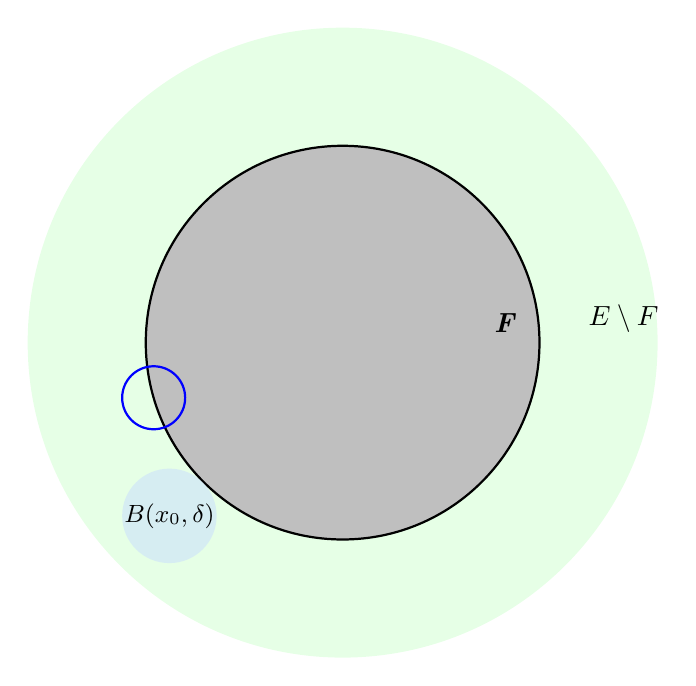
\begin{tikzpicture}
            % Define colors
            \definecolor{lightgreen}{RGB}{230, 255, 230}
            \definecolor{lightblue}{RGB}{200, 220, 255}
            \definecolor{darkgreen}{RGB}{0, 128, 0}

            % Large background circle
            \fill[lightgreen] (0, 0) circle (4cm);

            % Main circle
            \draw[thick, fill=lightgray] (0, 0) circle (2.5cm);
            \node[above right] at (1.8, 0) {\textbf{\textit{F}}};
            \node[above right] at (3, 0) {$E\setminus F$};

            % Small blue circle
            \draw[blue, thick] (-2.4, -.7) circle (0.4cm);

            % Highlighted area for excluded point
            \fill[lightblue, opacity=0.5] (-2.2, -2.2) circle (0.6cm);
            \node (_) at (-2.2, -2.2){\small $B(x_0, \delta)$};
        \end{tikzpicture}
        \caption{Un ensemble fermé\\
            \textit{À la borne, il est impossible de trouver une boules qui appartient à $F$, car il est impossible d'avoir une boule ouverte de  $r = 0$. Exemple: circle bleu foncé}\\
            \textit{Pour tout point dans $E \setminus F$ on peut trouver une boule ouverte}
        }
    \end{subfigure}
    \hfill
    \begin{subfigure}{0.45\textwidth}
        \centering
        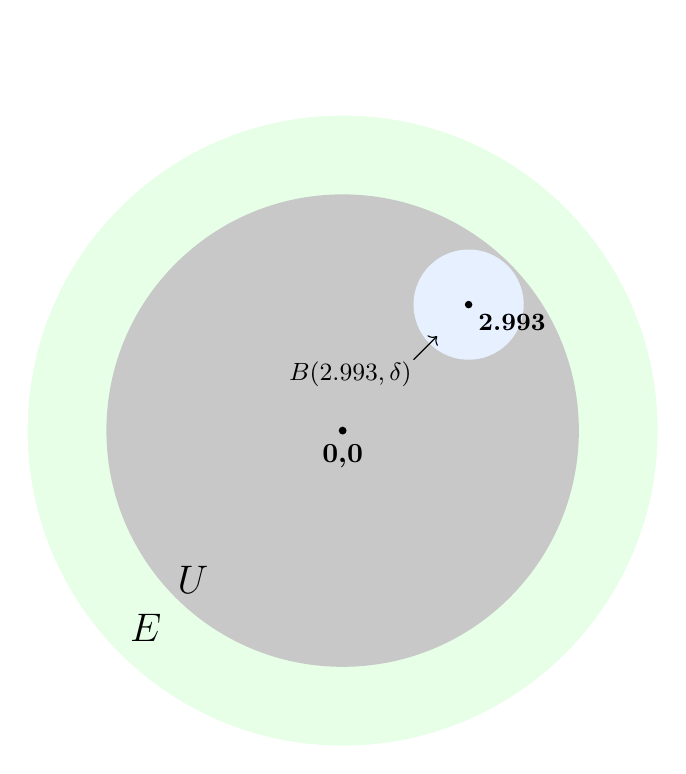
\begin{tikzpicture}
            % Define colors
            \definecolor{lightblue}{RGB}{230, 240, 255}
            \definecolor{lightgray}{RGB}{200, 200, 200}
            \definecolor{darkgreen}{RGB}{0, 128, 0}
            \definecolor{lightgreen}{RGB}{230, 255, 230}

            % Draw large circle
            \fill[lightgreen] (0, 0) circle (4cm);
            \fill[lightgray] (0, 0) circle (3cm);

            % Draw small circle
            \fill[lightblue] (1.6, 1.6) circle (0.7cm);
            \draw[fill=black] (1.6, 1.6) circle(0.4mm);
            \node[below right] at (1.6, 1.6) {\textbf{\small 2.993}};

            \draw[->] (0.9, 0.9)--(1.2, 1.2);
            \node[below left] (_) at (1, 1){\small $B(2.993, \delta)$};
            % Add points and labels
            \node[fill=black, circle, inner sep=1pt, label=below:{\textbf{0,0}}] at (0, 0) {};

            % Add text
            \node[right] at (1, 5) [align=left, text=darkgreen] {
                };
            \node (_) at (-1.9, -1.9){\Large $U$};
            \node (_) at (-2.5, -2.5){\Large $E$};
        \end{tikzpicture} 
        \caption{Un ensemble ouvert\\
            \textit{
                pour tout point pres de la borne
                on peut trouver une boule
                infiniment petite avec des
                points autour ce point inclu dans $U$.
            }
        }

    \end{subfigure}
    \caption{Démonstration des espaces ouverts et fermés}
\end{figure}

\begin{prop}.
    \begin{enumerate}
        \item 
            Une union des ensembles ouverts est aussi ouvert, idem avec l'intersection des ensembles ouverts. 
        \item  
            Une union des ensembles fermé est aussi fermé, idem avec l'intersection des ensembles fermé. 
    \end{enumerate}
\end{prop}

\section{Intérieur, adhérence, frontière}
Soit $A \subset E$. 
\begin{definition}
    Un point $x \in E$ est intérieur à $A$ s'il existe  $\delta > 0$ tel que  $B(x, \delta) \subset A$.\\
    Ensembles des points intérieur à $A$ se note  $Int(A)$ ou  $\mathring{A}$.
\end{definition}
\begin{intuition}
   $Int(A)$ est un ensemble qui est totalement dans  $A$ est se trouve loin des bords. 
\end{intuition}
\begin{tabular}[c]{@{}l@{}r@{}}
    \adjustbox{valign=t}{
    \parbox[t]{0.79\textwidth}{
    \begin{definition}
        Un point $x \in E$ est adhérent à  $A$ si  $\forall r > 0, \, B(x, r) \cap A \neq \O$ (toute boule centré dans $x$ intersecte  $A$).  \\
        Ensemble des points adhérents à $A$ se note  $Adh(A)$ ou  $\overline{A}$.
    \end{definition}
}
}
    &
    \hfill
    \adjustbox{valign=t}{
        \parbox[t]{0.2\textwidth}{
            \vspace{0.3cm}
    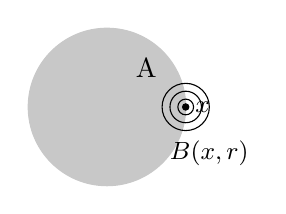
\begin{tikzpicture}
            \definecolor{lightgray}{RGB}{200, 200, 200}
        \filldraw[color=lightgray] (0,0) circle (1cm); 
        \coordinate (x) at (1, 0);
        \filldraw[color=black] (x) circle (0.4mm);
        \node[right] (_) at (x){\small $x$};
        \node (_) at (0.5, 0.5){A};

        \draw (x) circle (0.2cm);
        \draw (x) circle (0.3cm);
        \draw (x) circle (0.1cm);
        \node[below] (_) at (1.3, -0.3){\small $B(x, r)$};
    \end{tikzpicture} 
}
}
\end{tabular}
\begin{intuition}
   Si $A$ est ouvert (ses bords n'appartiennent pas à $A$), ses bords appartiennent à $Adh(A)$. Cette notion est utile pour completer des ensembles.
   \begin{eg}
       $\overline{\Q} = \R$ 
   \end{eg} 
\end{intuition}
\begin{definition}
    $Adh(A) \cap Adh(E \setminus A)$ est le bord de $A$ est s'appelle  la frontière de $A$.
\end{definition}
\section{Suite dans un éspace métrique}
\begin{definition}
    Une suite $(x_n)_{n \in \N}$ converge vers $x \in E$, si  $\forall \epsilon > 0, \exists N \in \N$ tel que :
    \[
    \forall n \ge N, \, d(x_n, x) \le  \epsilon
    \] 
\end{definition}
\begin{prop}
   Soit $A \in E$.\\ 
   \begin{enumerate}
       \item $x \in Adh(A)$ si et seulement si, il existe une suite $(x_n)_{n \in \N}$ d'éléments de $A$ telle que  $x_n \xrightarrow[n \to +\infty]{} x$ 
       \item $A$ est fermé (i.e contient sa frontière) si et seulement si la limite de toute suite  $(x_n)_{n \in \N}$ d'éléments de $A$ appartient à  $A$.
   \end{enumerate}
\end{prop}
\begin{intuition}
   \begin{enumerate}
       \item Si $(x_n)_{n \in \N}$ est d'éléments de  $A$ ($\forall n \in N, \, x_n \in A$), donc elle converge vers un éléments $x$ qui peut être soit dans  $A$, soit la borne des éléments de  $A$, alors à la frontière. 
       \item Si la limite de toute suite $(x_n)_{n \in \N}$ des éléments de  $A$ est aussi dans  $A$, alors la frontière de  $A$ est inclu dans  $A$. Car l'une des suites tend vers la borne.
   \end{enumerate} 
\end{intuition}
\begin{definition}
    Une suite $(x_n)_{x \in \N}$ est de Cauchy si  $\forall \epsilon > 0, \exists N \in \N$ tel que:
    \[
    \forall n, p \ge N, \, d(x_n, x_p) \le \epsilon
    \] 
\end{definition}
\begin{intuition}
   Une suite de Cauchy c'est comme on mesure un point et on le localise, i.e:
   \begin{enumerate}
       \item On dit qu'il est entre $0$ et  $1$.
       \item Ensuite, on precise plus et on dit qu'il est entre  $0.5$ et  $0.6$.
       \item Puis, entre  $0.55$ et  $0.56$
   \end{enumerate}
   On peut infiniment augmenter le niveau de précision. C'est ça l'idée d'une suite de Cauchy.
\end{intuition}
\begin{definition}
    Un éspace métrique $(E, d)$ est \textbf{complet} si toute suite  $(x_n)_{n \in \N}$ d'éléments de  $E$ converge vers une limite  $x$ qui appartient aussi à  $E$.
\end{definition}
\begin{eg}
    Un éspace métrique $(]0, 1], d)$ avec $d$ une distance euclidienne n'est pas complet, car  soit une suite: $x_n = \frac{1}{n}$ dont la limite est $0$. Par contre,  $0 \not\in ]0, 1]$. Donc cet éspace n'est pas complet. 
\end{eg}
\begin{figure}[h]
   \centering 
   \begin{tikzpicture}
       \draw[->] (-1, 0) -- (2, 0); 
       \node[below] (_) at (2,0){$x$};

       \node (_) at (0,0){]};
       \node[below] (_) at (0,-0.3){$0$};
       \node (_) at (1,0){]};
       \node[below] (_) at (1,-0.3){$1$};
       \draw[color=red] (0,0)--(1,0);
   \end{tikzpicture}
   \caption{$(]0, 1], d)$ n'est pas complet}
\end{figure}
\begin{eg}
   Un éspace $(\Q, d)$ n'est pas complet. Car on peut prendre une suite  $x_n$ tendant vers  $\sqrt{2} \not\in \Q$.
\end{eg}

\begin{figure}[H]
    \centering
    \incfig{q_not_complete}
    \caption{$\Q$ pas complet}
    \label{fig:q_not_complete}
\end{figure}

\begin{definition}
    Soit une suite $(x_n)_{n \in \N}$ et une application  $\phi:\N \to \N$ \underline{strictement croissante}. Une suite $(x_n)_{\phi(n)}$ est appellée une sous-suite.
\end{definition}
\begin{eg}
    Soit une application $\phi: \N \to \N$ telle que $\phi(n) = 2n$. Donc  $(x_n)_{\phi(n)}$ est une sous-suite de  $(x_n)_{n \in \N}$ et:
    \[
        (x_n)_{\phi(n)} = \{x_0, x_2, x_4, \ldots\}
    \] 
\end{eg}

\section{Compacité}
\begin{definition}
    Soit $F \subset E$. Un \textbf{recouvrement ouvert} de $F$, est une union des enesembles ouverts:  $\bigcup_{i \in I} U_i$ tel que $F \subset \bigcup_{i \in I} U_i$
\end{definition}
\begin{eg}
    Soit $F = ]0, 1[$. Soit $A = \left\{]\frac{1}{n}, 1 + \frac{1}{n}[, n \in N\right\}$. $F \subset \bigcup_{n \in N^{*}} A_n$ i.e union infinie des $A_i$ couvre $F$.
\end{eg}
\begin{definition}
    Un ensemble $F \subset E$ est \textbf{compact} si \underline{pour tout} recouvrement ouvert, i.e \underline{pour tout} union des ensembles ouvert $\bigcup_{i \in I} U_i$ qui couvre $F$, on peut prendre un nombre \underline{fini} des  $U_i$ et couvrir $F$.
\end{definition}
\begin{theorem}
    Un ensemble $K \subset E$ est compact, si toute suite $(x_n)_{n \in \N}$ des éléments de $K$, possede une sous-suite qui converge  vers un éléments $x \in K$.
\end{theorem}
\begin{intuition}
    S'il existe tel suite $(x_n)_{n \in \N}$ sans sous-suite convergente vers un éléments de  $K$, donc les valeurs sont en-dehors de  $K$ et donc il existe un ensemble qui couvre $K$  seulement avec un nombre infini des ensembles. 
\end{intuition}
Pourquoi a-t-on besoin de compacité? Car cela nous donne une
\begin{prop}
    Si $K \subset E$ est compact, alors $K$ est fermé et borné.\\
    Si $K$ est compact est  $F$ est borné, donc  $K \cap F$ est compact\\
    Si $K$ est compact, donc  $K$ est complet
\end{prop}
\begin{property}
    La différence entre \textit{compacité} et {complecité}:
    \begin{itemize}
        \item complecité nous assure qu'il n'y a pas de trou dans un espace
        \item compacité nous assure qu'un ensemble est fermé et borné
    \end{itemize}
\end{property}
\section{Limites et applications continues}
2



\nocite{*}
\printbibliography


\end{document}

